\subsection{Overview}
CLup's architecture is layered as follows:
\begin{itemize}
	\item \textbf{Presentation layer} (P) handles the interaction with users. It contains the interfaces able to communicate with them and it is responsible for rendering of the information. Its scope is to make understandable the functions of the application to the customers.
	\item \textbf{Application layer} (A) takes care of the functions to be provided for the users. It also coordinates the work of the application, making logical decisions and moving data between	the other two layers.
	\item \textbf{Data access layer }(D) which takes care of the information management, database access control. It also handles data retrieval and passes them to upper level layers.
\end{itemize}
 
The architecture style chosen for CLup is the \textbf{multi-tier} one.
As previously anticipated in the Requirements Analysis and Specifications Document, there will be at least one server for each one of the following interest areas:
\begin{itemize}
    \item Bookings
    \item Queues
    \item Notifications
    \item Stores
    \item Staff members
    \item Customers
\end{itemize}

This is mainly done to distribute workload as well as making the overall system more robust.

There will be also at least two servers for the two following functionalities:
\begin{itemize}
    \item Customer related functionalities
    \item Staff related functionalities
\end{itemize}
The bookings, queue and notifications databases will be distributed and replicated all over the entire store list. Each store will have its own instance of bookings, queue and notifications database while a central logic server will act as a request redirector towards them whenever needed.\\

In Figure \ref{fig:HLArch} is represented the high-level architecture of the system: customers clients, through an internet connection, can connect to CLup's App Servers, which represent the A layer of the Clup customer side. Client's operations store o retrieve information from People DB Servers or directly from the Local DB of the store, depending by the kind of information. Staff clients instead are connected through a LAN connection to their Local Web Server, who will redirect their requests to the Staff Operations Manager server. This machine is expected to process the logic of requests and then submit them to the Local Application server who also store or retrieve the information from the Local DB or People DB server depending by the situation. Local Application Server is fundamental also for Totem users, in fact the Totem rely on this server for its requests. Staff clients may need to connect to Clup Centralized Hardware, to do this they need an internet connection to get in contact with the dedicated Central Web server, the P layer who then send the request to the Store Operations Manager, the A layer. This server stores and retrieves information from Stores DB servers

\begin{figure}[h!]
	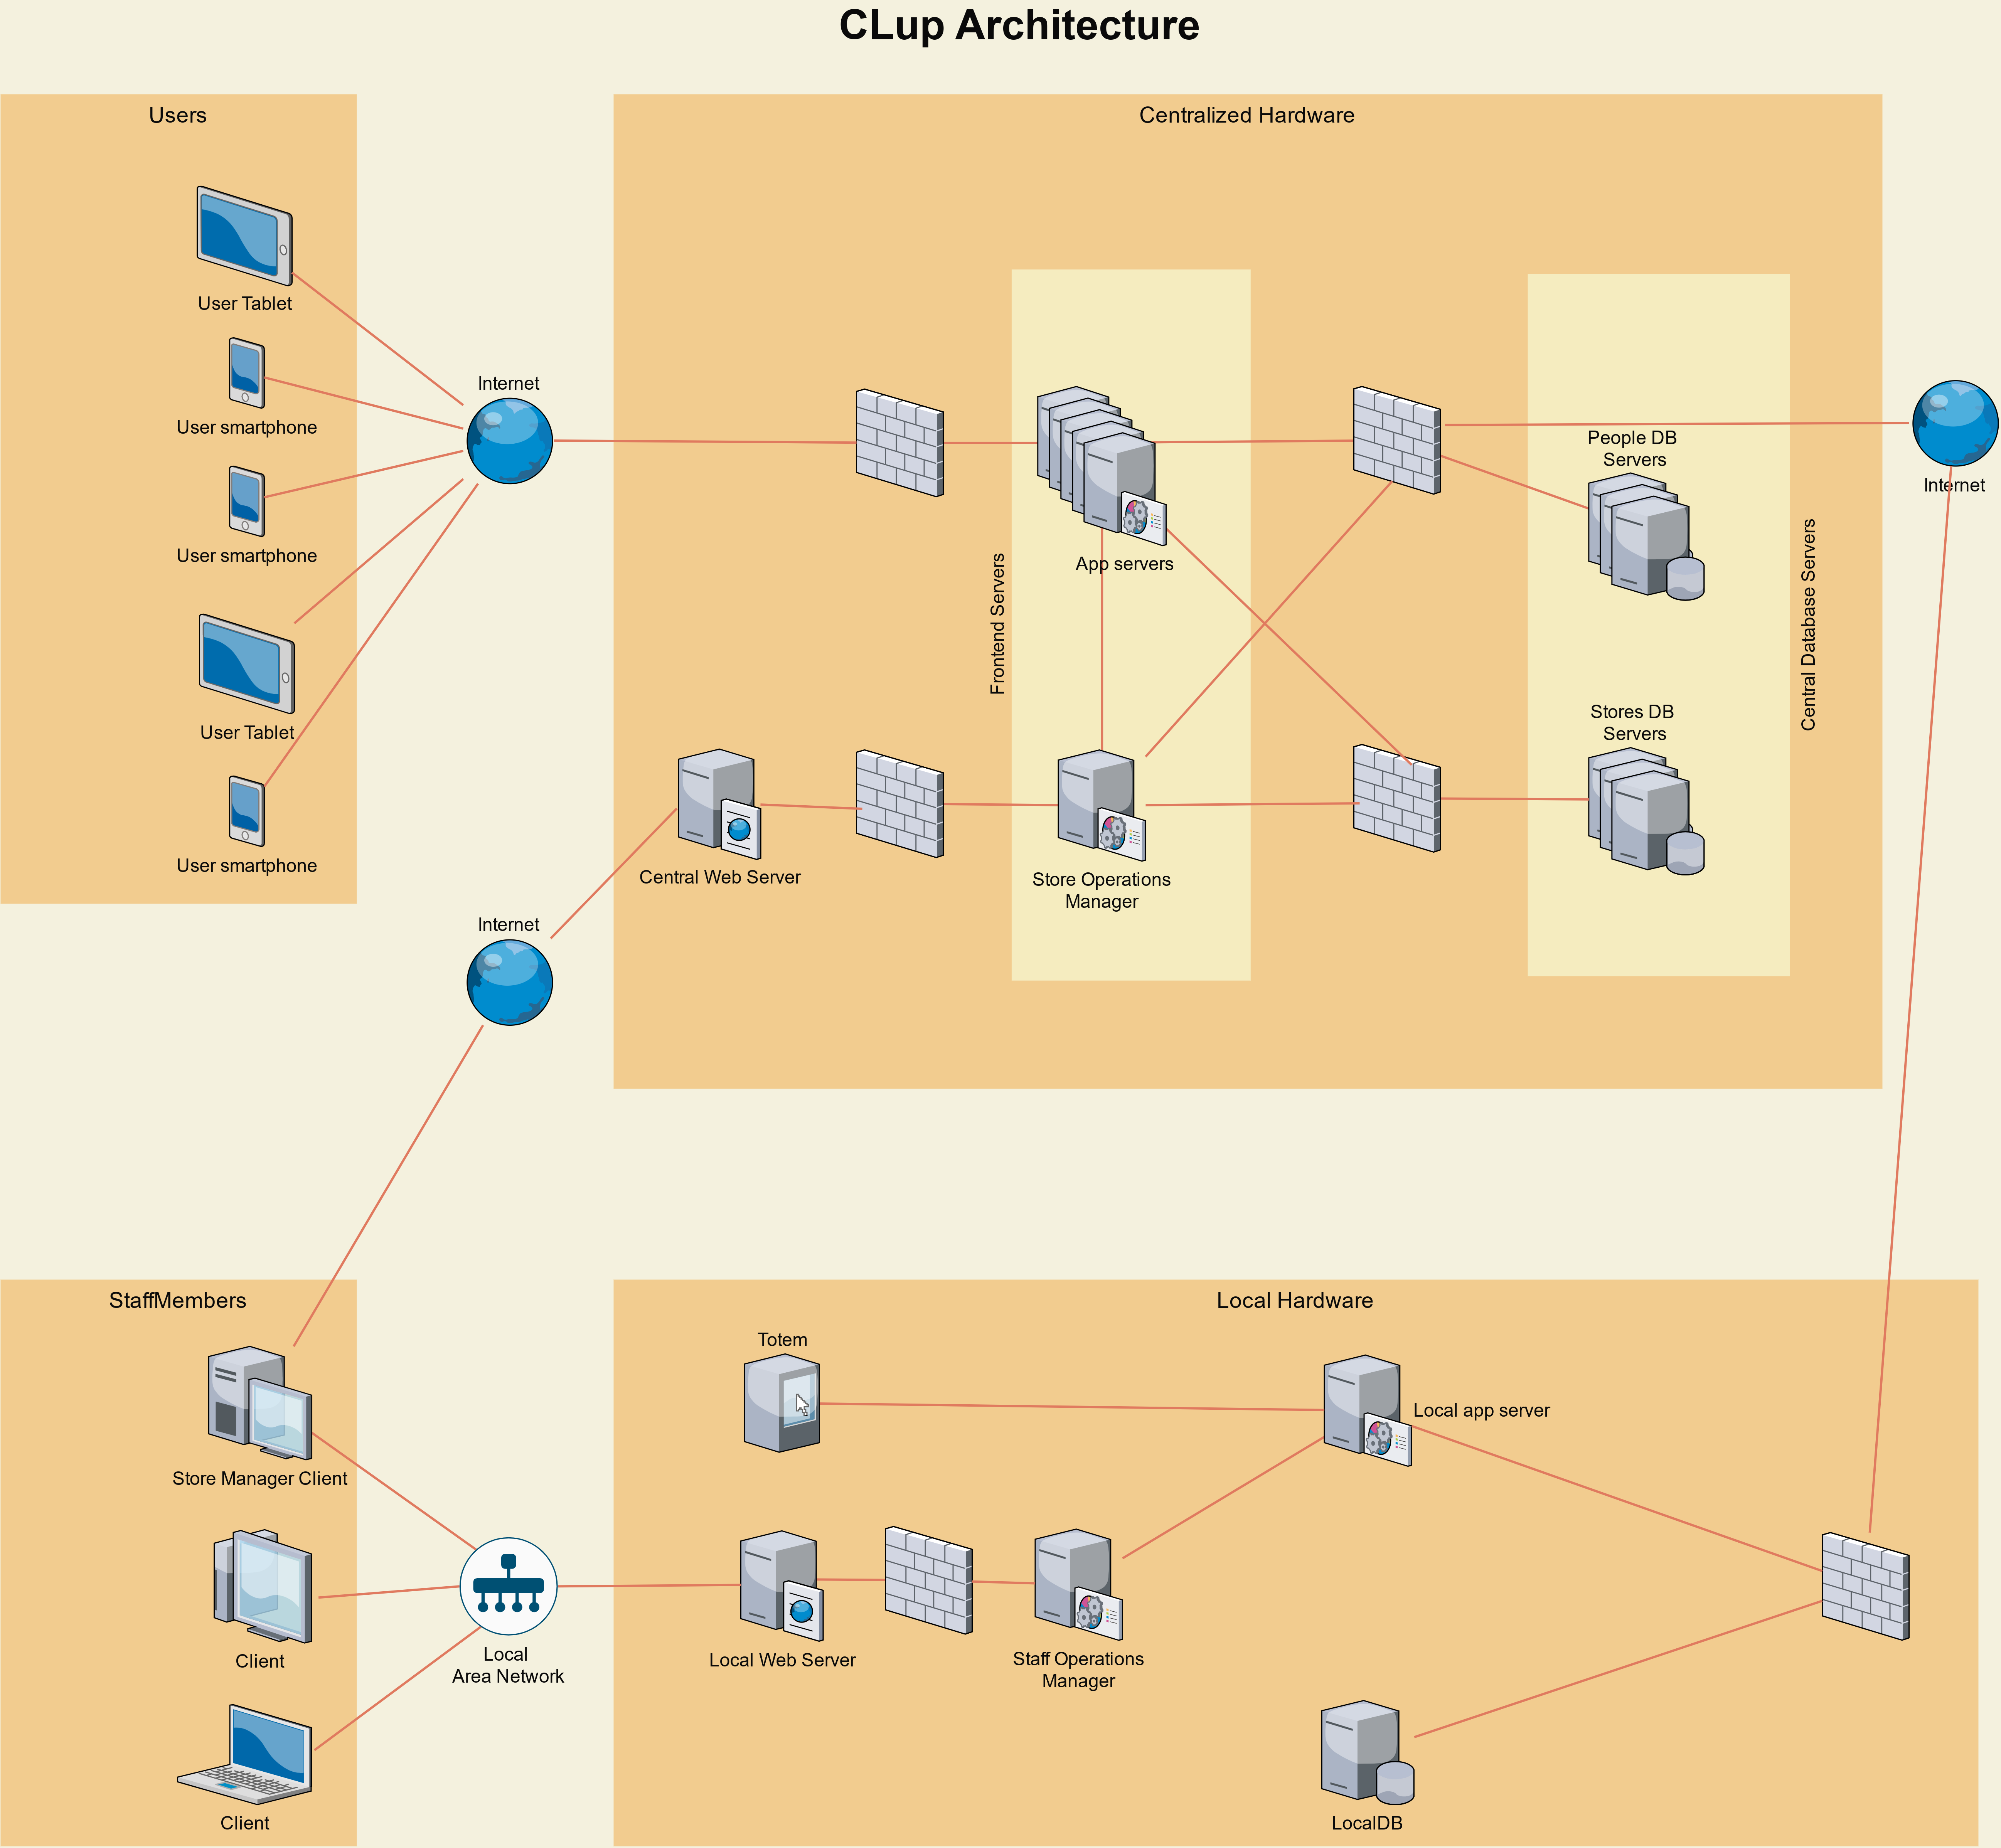
\includegraphics[width=\linewidth]{../Diagrams/Archtecture/Architecture_diagram.png}
	\caption{High-level architecture}
	\label{fig:HLArch}
\end{figure}
\newpage
\subsection{Component view}
\begin{landscape}
\begin{figure}[H]
	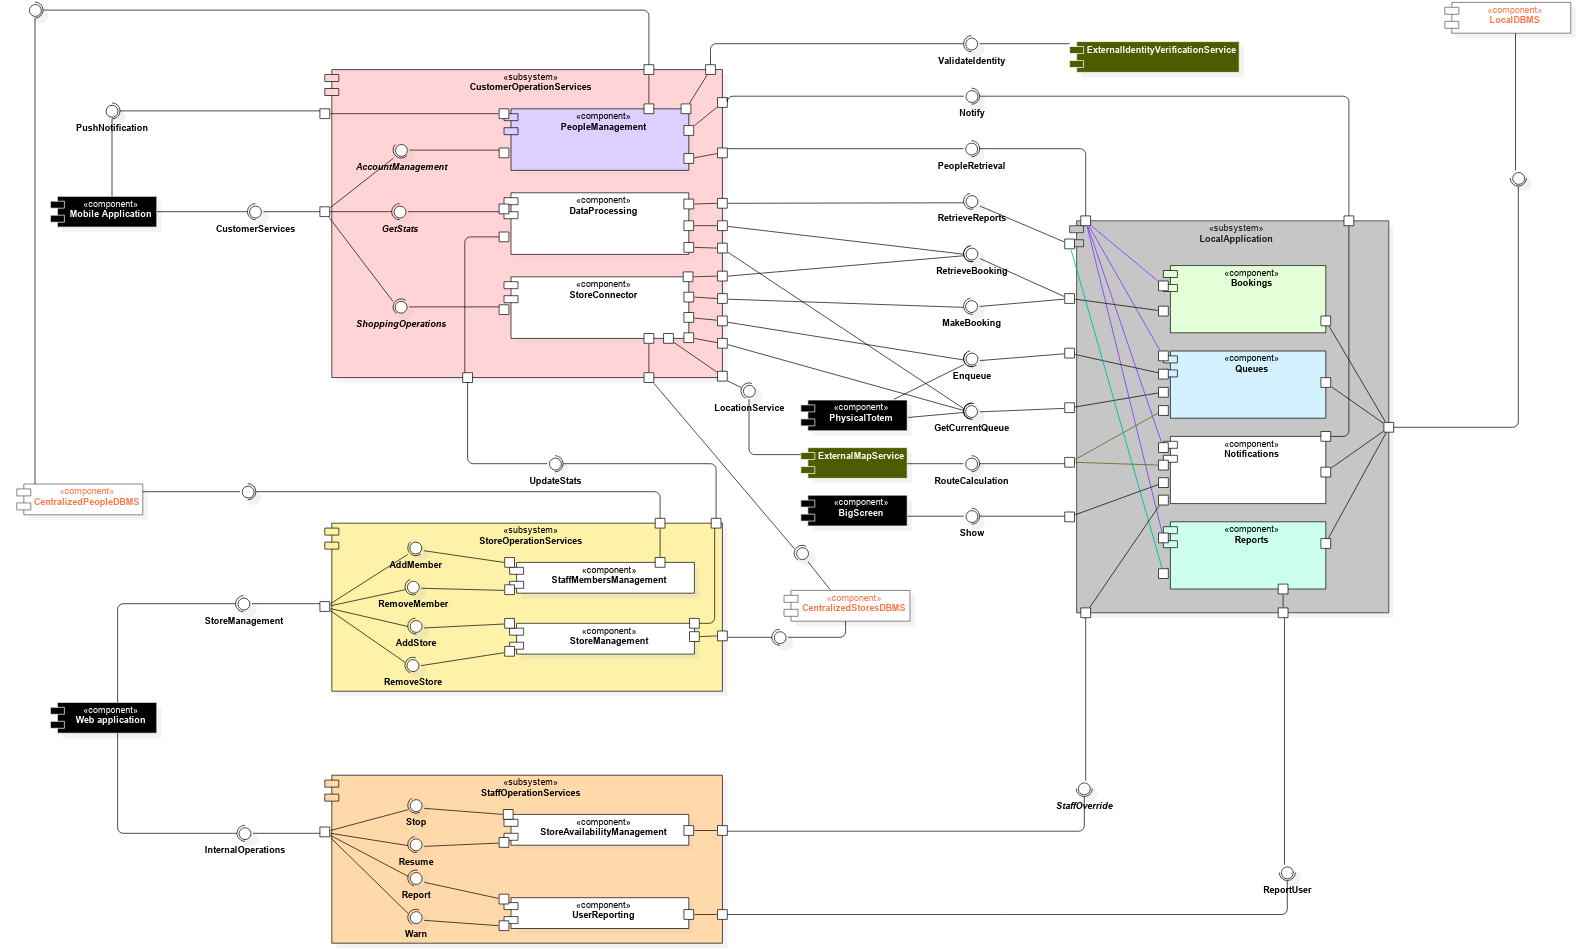
\includegraphics[width=\linewidth]{../Diagrams/ComponentDiagram.png}
	\caption{Component Diagram}
	\label{fig:CompDgm}
\end{figure}
\end{landscape}
In Figure \ref{fig:CompDgm} is represented the component diagram of the internal structure Application layer, showing how its components and subsystems interact. As previously said, the A layer contains Clup's functional business logic which drives the application’s core capabilities, it builds  a bridge between the presentation layer and the data layer. What follows is a brief description of every component and subsystem:
\begin{itemize}
	\item \textbf{Staff Operation Services}: This subsystem contains 2 components:
	\begin{itemize}
		\item \textbf{Store Availability Management}: This is the component responsible for both interruption and recovery of availability of a store to accept new virtually queued customers
		\item \textbf{User Reporting}: This component's function is to take note of customers bad behaviours 
	\end{itemize} 

	\item \textbf{Store Operation Services}: This subsystem contains 2 components:
	\begin{itemize}
		\item \textbf{Staff Members Management}: A subscribed store can grant access and credentials to CLup's store services through this component 
		\item \textbf{Store Management}: A store can enroll to CLup's network through this component
	\end{itemize} 

	\item \textbf{Customer Operation Services}: This subsystem has 2 subcomponents
	\begin{itemize}
		\item \textbf{People Management}: This component is responsible for customers subscription, login t CLup and, thanks to the association device-person, notifications by CLup and Supermarkets
		\item \textbf{Data Processing}: As the name suggests, the Data Processing component takes care of data about availability of stores, time slots and queues status. It also evaluate time slots, days and store crowdness level and infer better solutions.
		\item \textbf{Store Connector}:this component acts as an interface towards the distributed part of the application and its components. It allows the reaching of and use of store-hosted components such as Bookings, Queues.
	\end{itemize}

	\item \textbf{Local Application }:
	\begin{itemize}
		\item \textbf{Bookings}: This component makes possible booking an entrance, it takes care of the logic of the booking procedure and retrieves information of a previously made reservation
		\item \textbf{Queues}: This is the component responsible for the basic function of CLup, it has read-write access to stores queues and allows also to block and unblock them
		\item \textbf{Notifications}: Here is were all kind of users notifications are generated
		\item \textbf{Reports}: This is the component that instead generate bad behaviours reports
	\end{itemize}
	\item \textbf{External Map Services}: This is the component that provides the map interface
	\item \textbf{Physical Totem}: This component is a simplified version of the mobile app, it has only what is needed to perform the basic function.
\end{itemize}

\subsection{Deployment view}
\begin{figure}[H]
	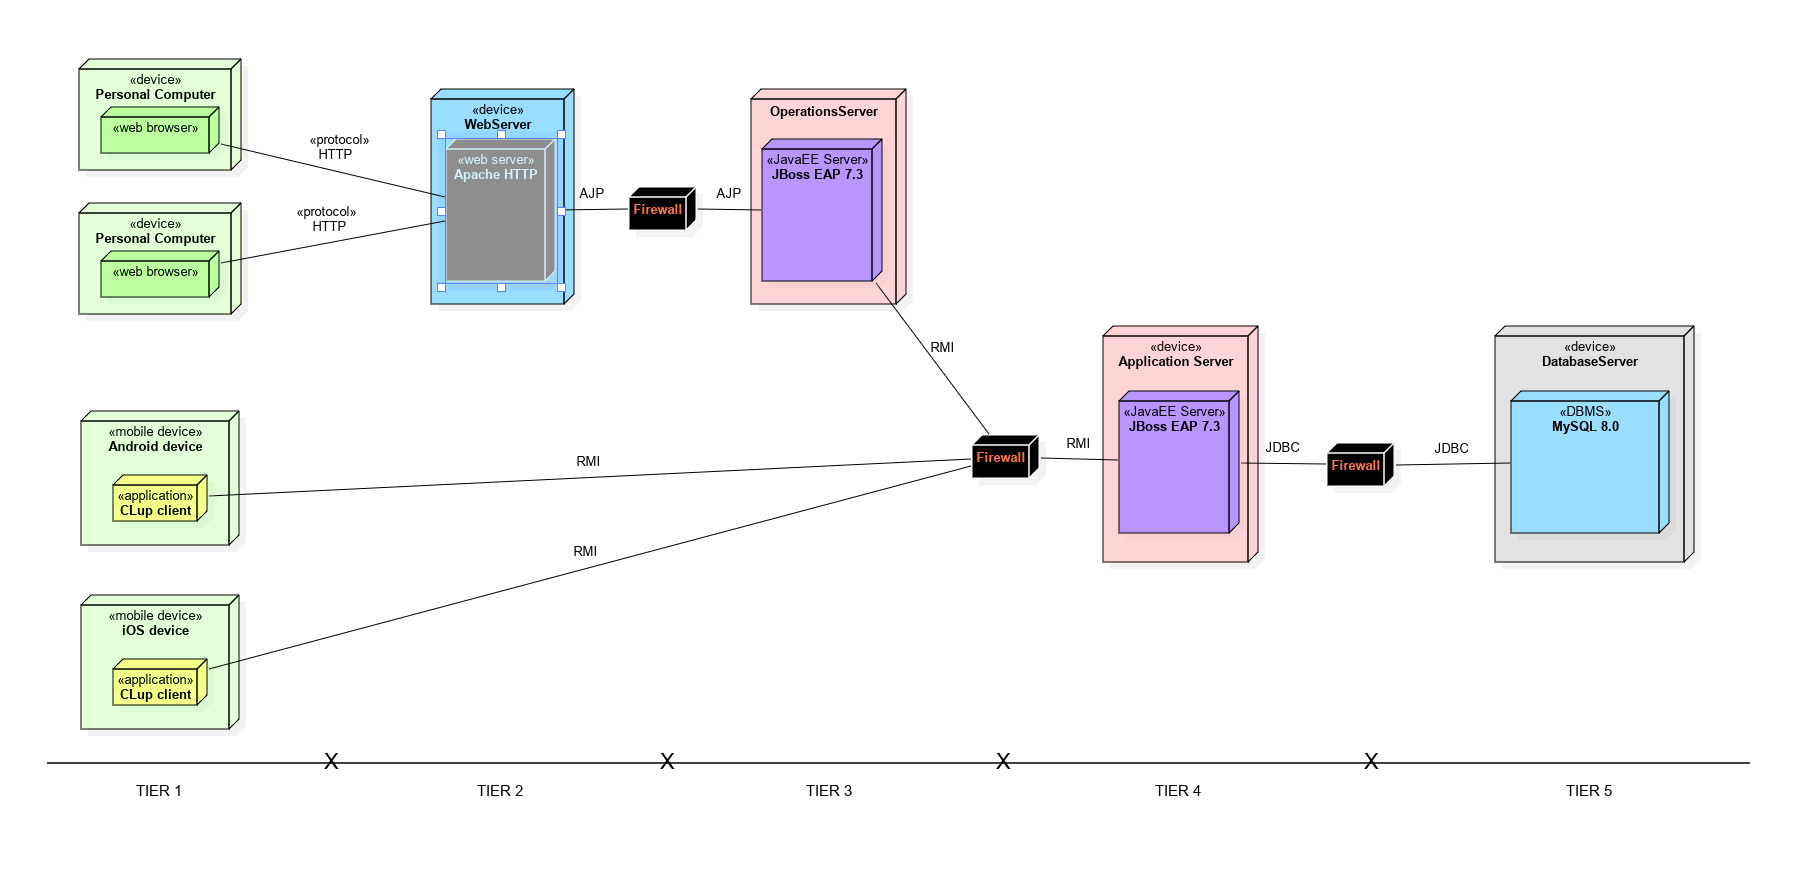
\includegraphics[width=\linewidth]{../Diagrams/deployment_diagram.png}
	\caption{Deployment Diagram}
	\label{fig:DEPL}
\end{figure}
\textbf{CLup} is designed according to a \textbf{multi-tier architecture} approach, which is represented by figure \ref{fig:DEPL}. Given the heavy distribution adopted for the logical layer of the application, a simplified view is depicted.
\begin{itemize}
    \item \textbf{Tier 1}: the \textit{client tier} includes everything from a smartphone to a desktop computer, mobile devices being the target for end-users while desktop/office PCs for stores staff members. 
    \begin{itemize}
        \item Mobile CLup applications connect to the main application servers via RMI
        \item Desktops/office PCs use a standard web application, which offers mainly static content.
    \end{itemize}
    \item \textbf{Tier 2:} the \textit{web tier} offer standard web server functionality. An \textbf{Apache} Server takes care of the HTTP requests from the staff's office computers. It then forwards them to application servers by using the \textbf{Apache JServ Protocol} (AJP)
    \item \textbf{Tier 3:} the \textit{operations tier} serves as main interface between the outer levels and the inner ones, by accepting incoming requests and redirecting them to the appropriate inner components when necessary. This layer is staff-operations only, and is particularly aimed at reducing main servers' workload by further distributing tasks. A \textit{JBoss EAP server} is run to accomplish this tier's tasks, and it communicates with inner level servers via RMI.
    \item \textbf{Tier 4}: the application tier is the core of CLup functionality. It includes the greatest majority of logical functionality (customer functionalities for the most part) and - architecturally wise - it's distributed across multiple servers: some centralized, some others distributed as one per each physical store. Each of those runs a JBoss EAP server. 
    \item \textbf{Tier 5}: the last and innermost tier, the \textit{data tier}, handles data management and retrieval. It's controlled by tiers 3 and 4, and it's invoked by use of the \textbf{Java DataBase Connectivity} APIs (JDBC). \textbf{MySQL} has been chosen for this Tier.

\end{itemize}

\subsection{Runtime view}
The following diagrams (\textit{UML sequence\footnote{As per \cite{UML:ref}}}) aim at giving an overall view about the main components interactions in the real world. Side-interest, particular cases or situations have been left uncovered for clarity and focus reasons. For the same reasons, some \textit{notation abuses} may have been made regarding the main component in each diagram and its lifeline/messages back to the requester.\newline


\noindent{\color{gray}
\fbox{%
    \parbox {\textwidth}{%
        \small
        You will find reference to undefined methods and interfaces inside the diagrams of this sections. Those diagrams are to be intended as a guideline for the Developers, to help them better visualize the core design choices made. They do \textbf{not} represent the final implementation result nor intend to irrevocably specify its characteristics.

    }%
}}


\paragraph{Store Operations}
We can see in these diagrams the whole CLup architecture at work. A qualified member of the store's staff can, after strong authentication (not depicted), invoke the stop and resume of the store's operation. The first meaning no more customers allowed inside the store, no more physical tickets being issued at the totems, and eventually notifications being dispatched to the affected customers\footnote{Refer to \ref{affected:def} \space for details}; the second implying correct and complete resuming of the store functionality. See figures \ref{fig:sStoreRes} and \ref{fig:sStoreOver}.

\paragraph{Registration and sign-up }
Here we can see the different components involved in the signing up process of customer as opposed to stores' staff members, or store themselves. Different components at different locations are used in each case. See figures \ref{fig:sCusSign}, \ref{fig:sStoreEn} and \ref{fig:sStaffEn}.

\paragraph{Tickets and Booking}
The core of CLup's functionality. We can see how these features involve both centralised and remote (localized) servers to work. See figures \ref{fig:sCusBook} \space and \ref{fig:sCusEnq}. \newline
See also \ref{fig:sTotemEnq} regarding offline, physical tickets issuing.

\paragraph{Reporting and Warning}
Finally, the reporting \& warning functionalities of CLup. They allow CLup (automatically) and stores' staff to inform users about relevant events, or even reporting them for misbehaviours. See figures \ref{fig:sUserRep}, \ref{fig:sUserWarn}.

\begin{figure}[H]
	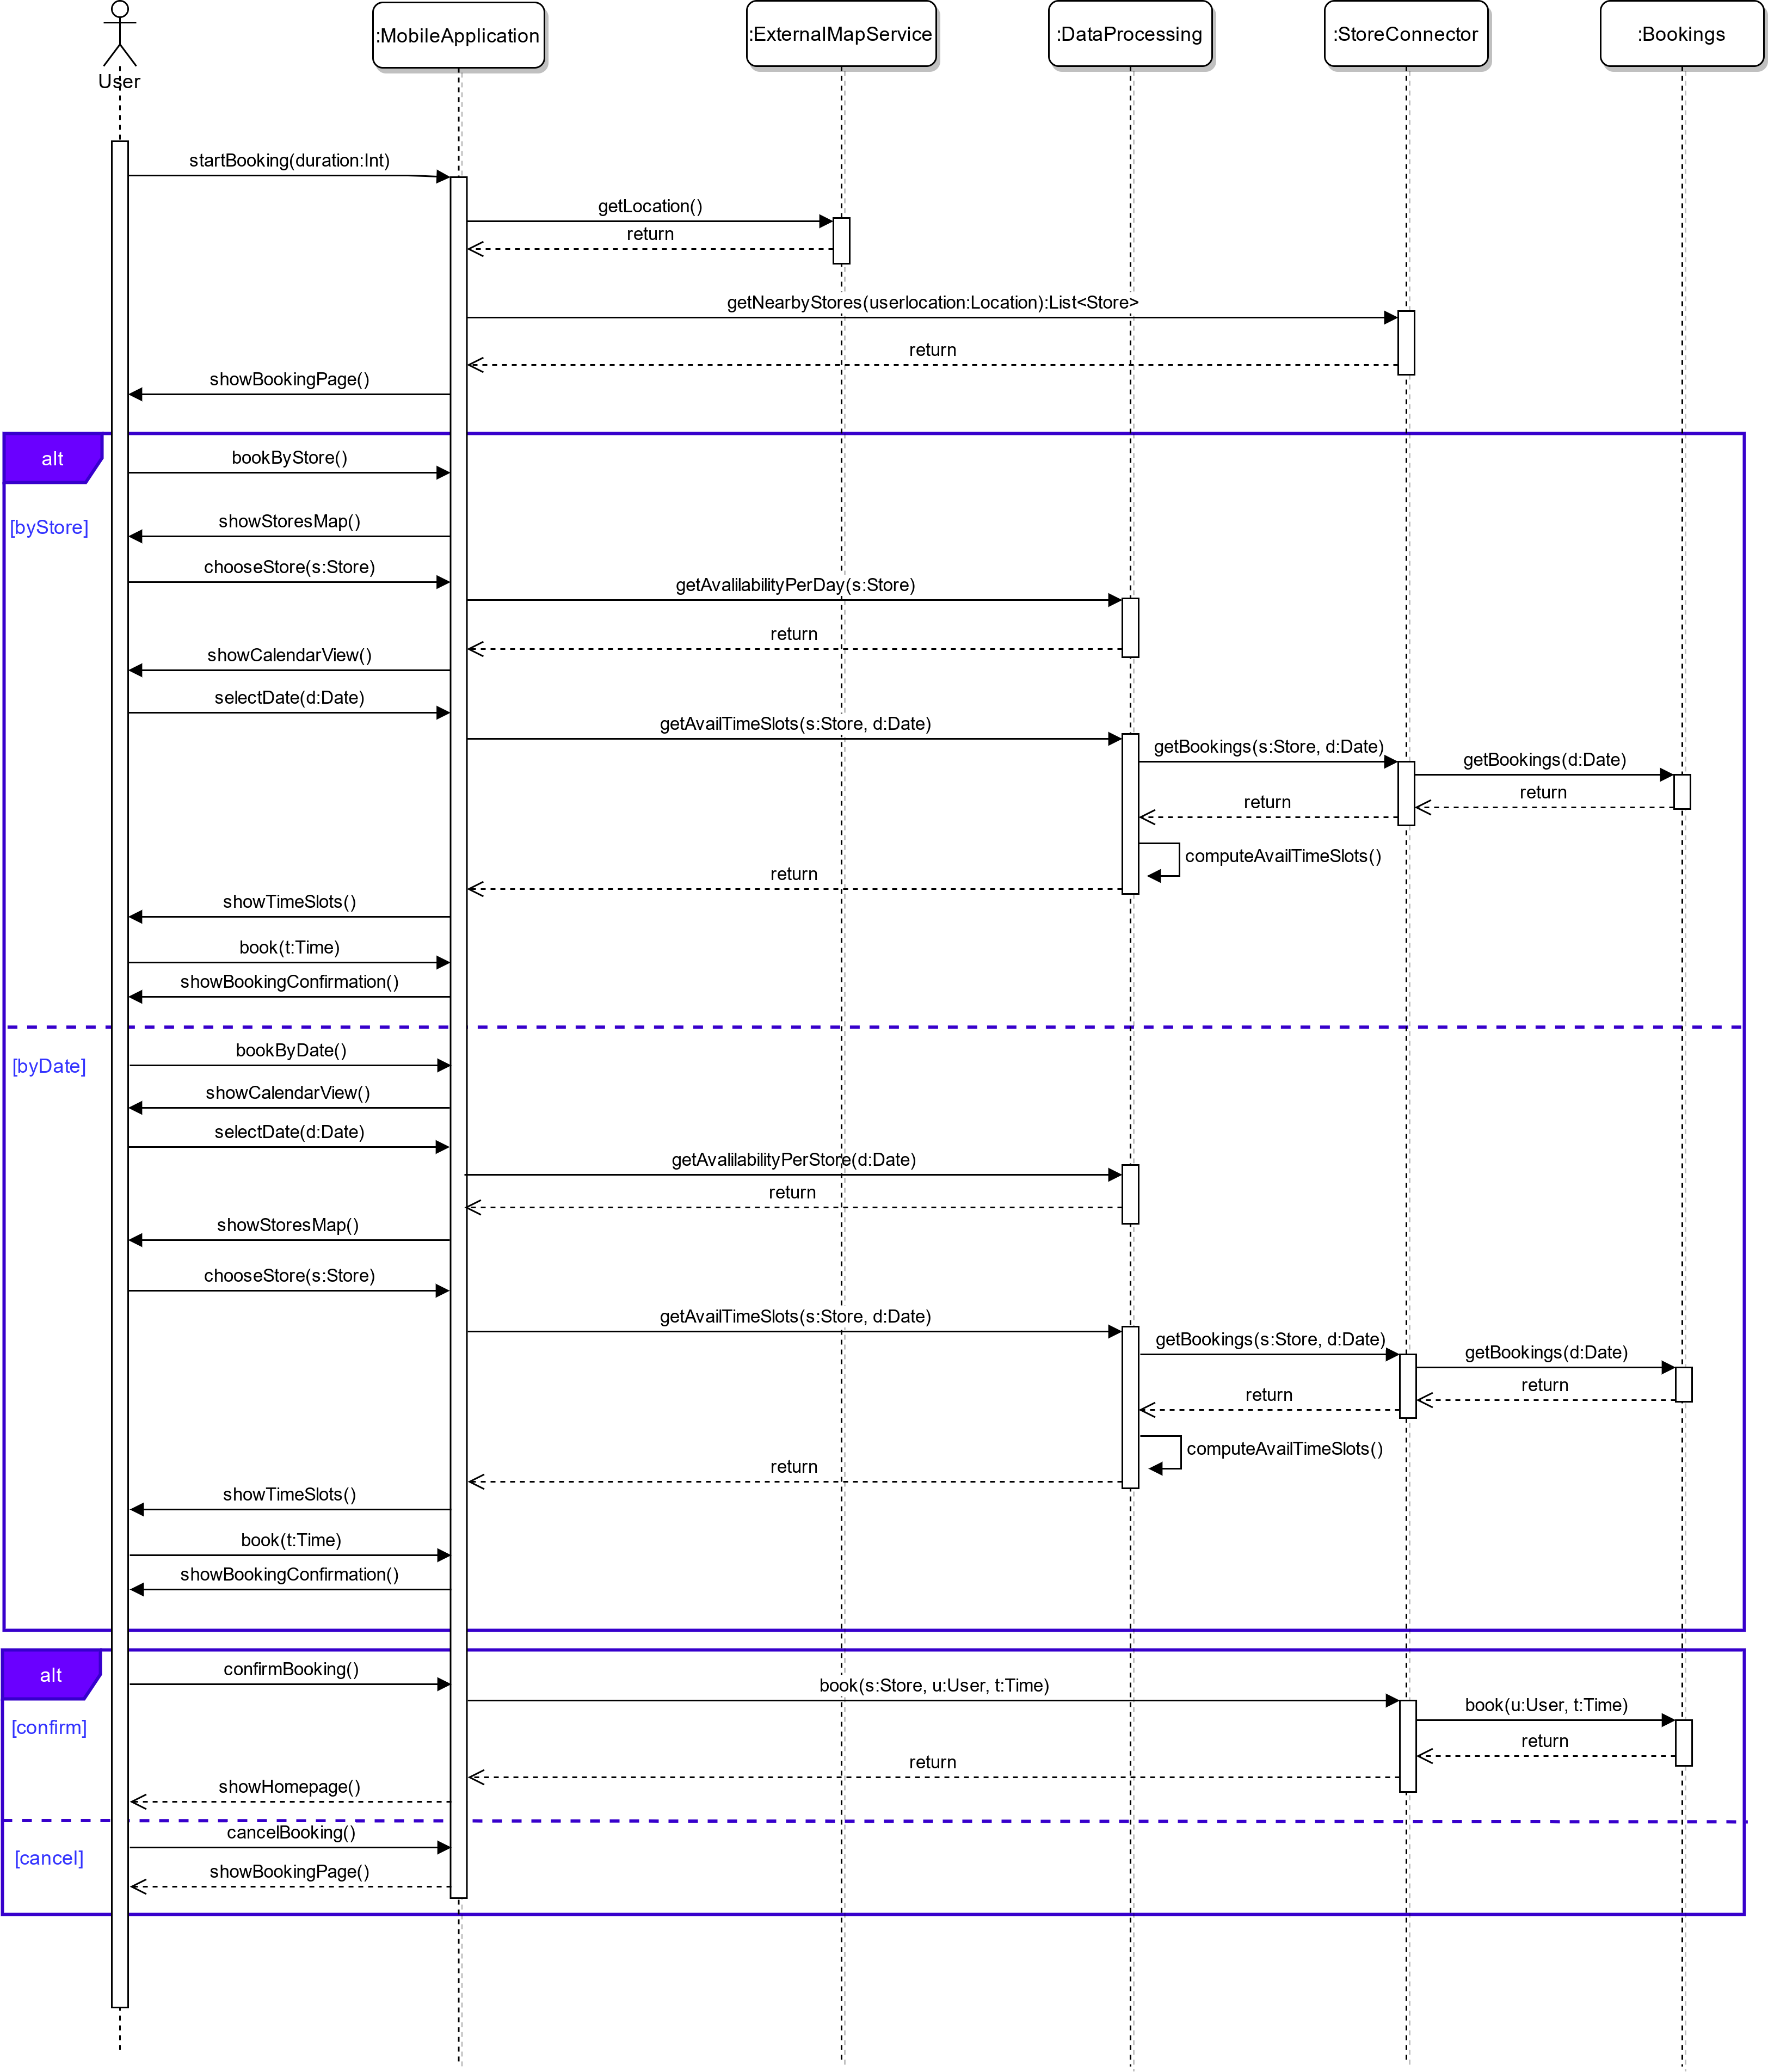
\includegraphics[width=\linewidth]{../Diagrams/Sequence/sequence_customer_book.png}
	\caption{Sequence Diagram: Customer Booking procedure}
	\label{fig:sCusBook}
\end{figure}

\begin{figure}[H]
	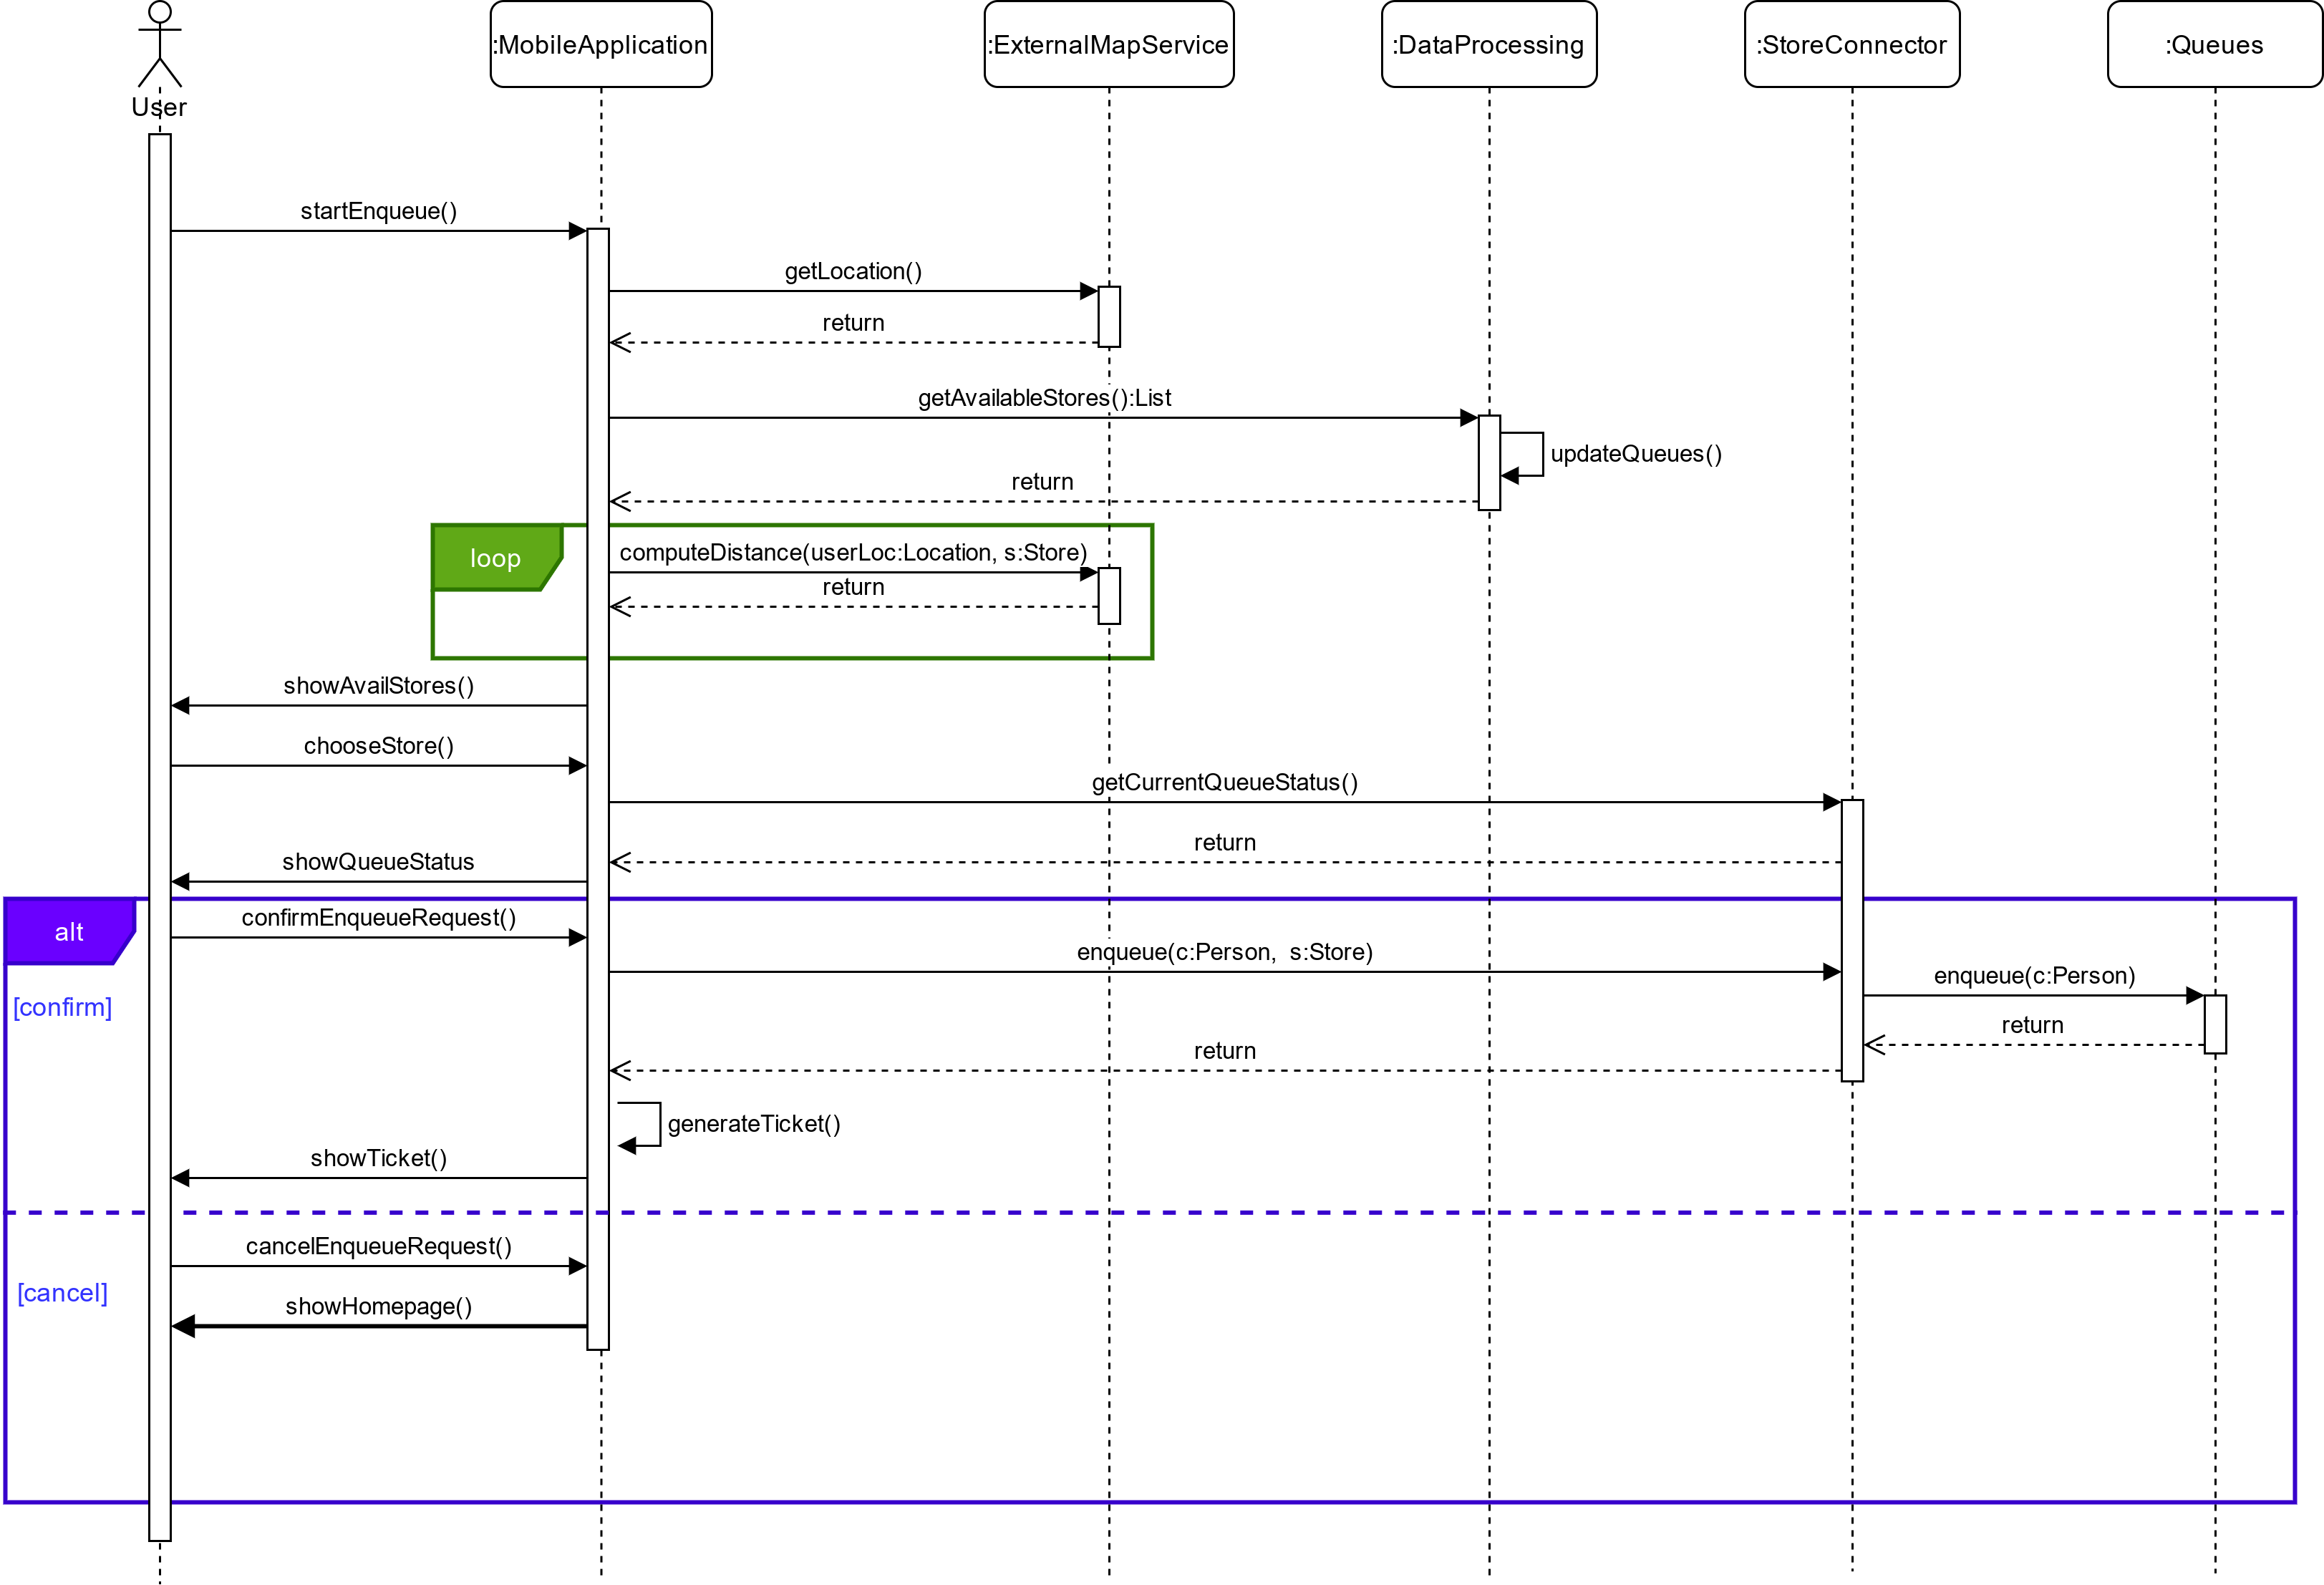
\includegraphics[width=\linewidth]{../Diagrams/Sequence/sequence_customer_enqueue.png}
	\caption{Sequence Diagram: Customer Enqueue (virtual ticket) procedure}
	\label{fig:sCusEnq}
\end{figure}

\begin{figure}[H]
	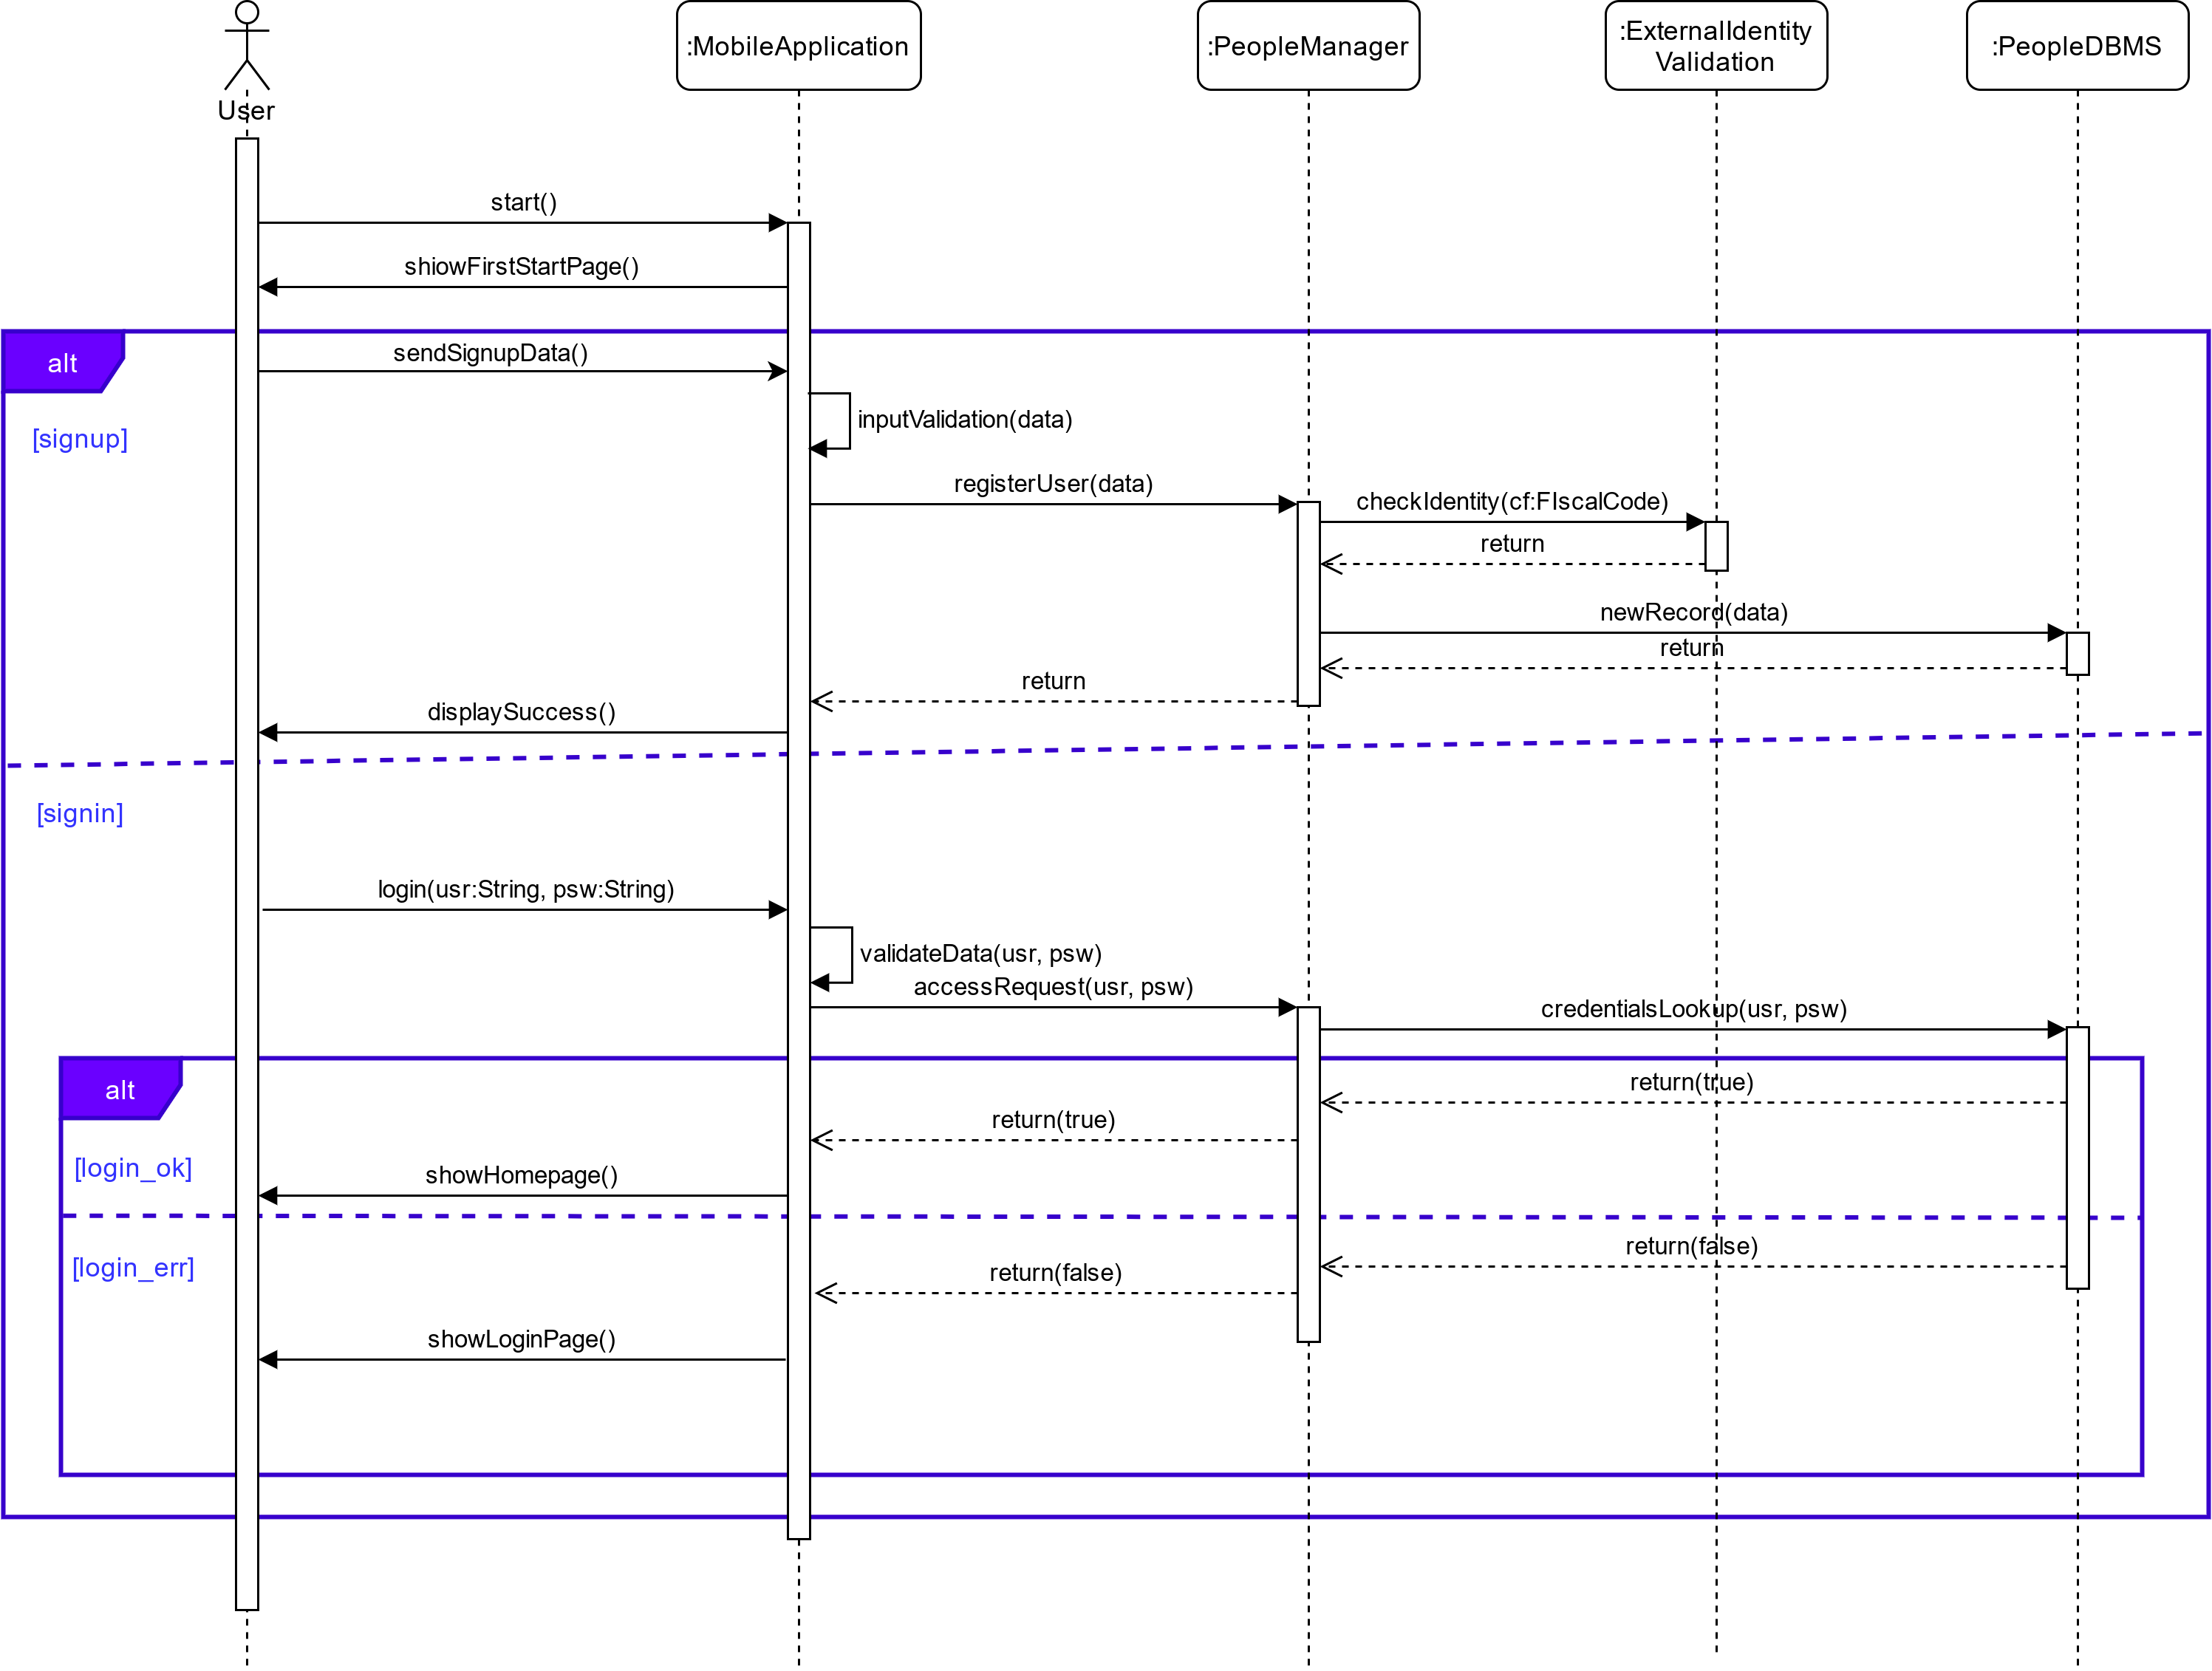
\includegraphics[width=\linewidth]{../Diagrams/Sequence/sequence_customer_signup.png}
	\caption{Sequence Diagram: Customer Sign-up procedure}
	\label{fig:sCusSign}
\end{figure}

\begin{figure}[H]
	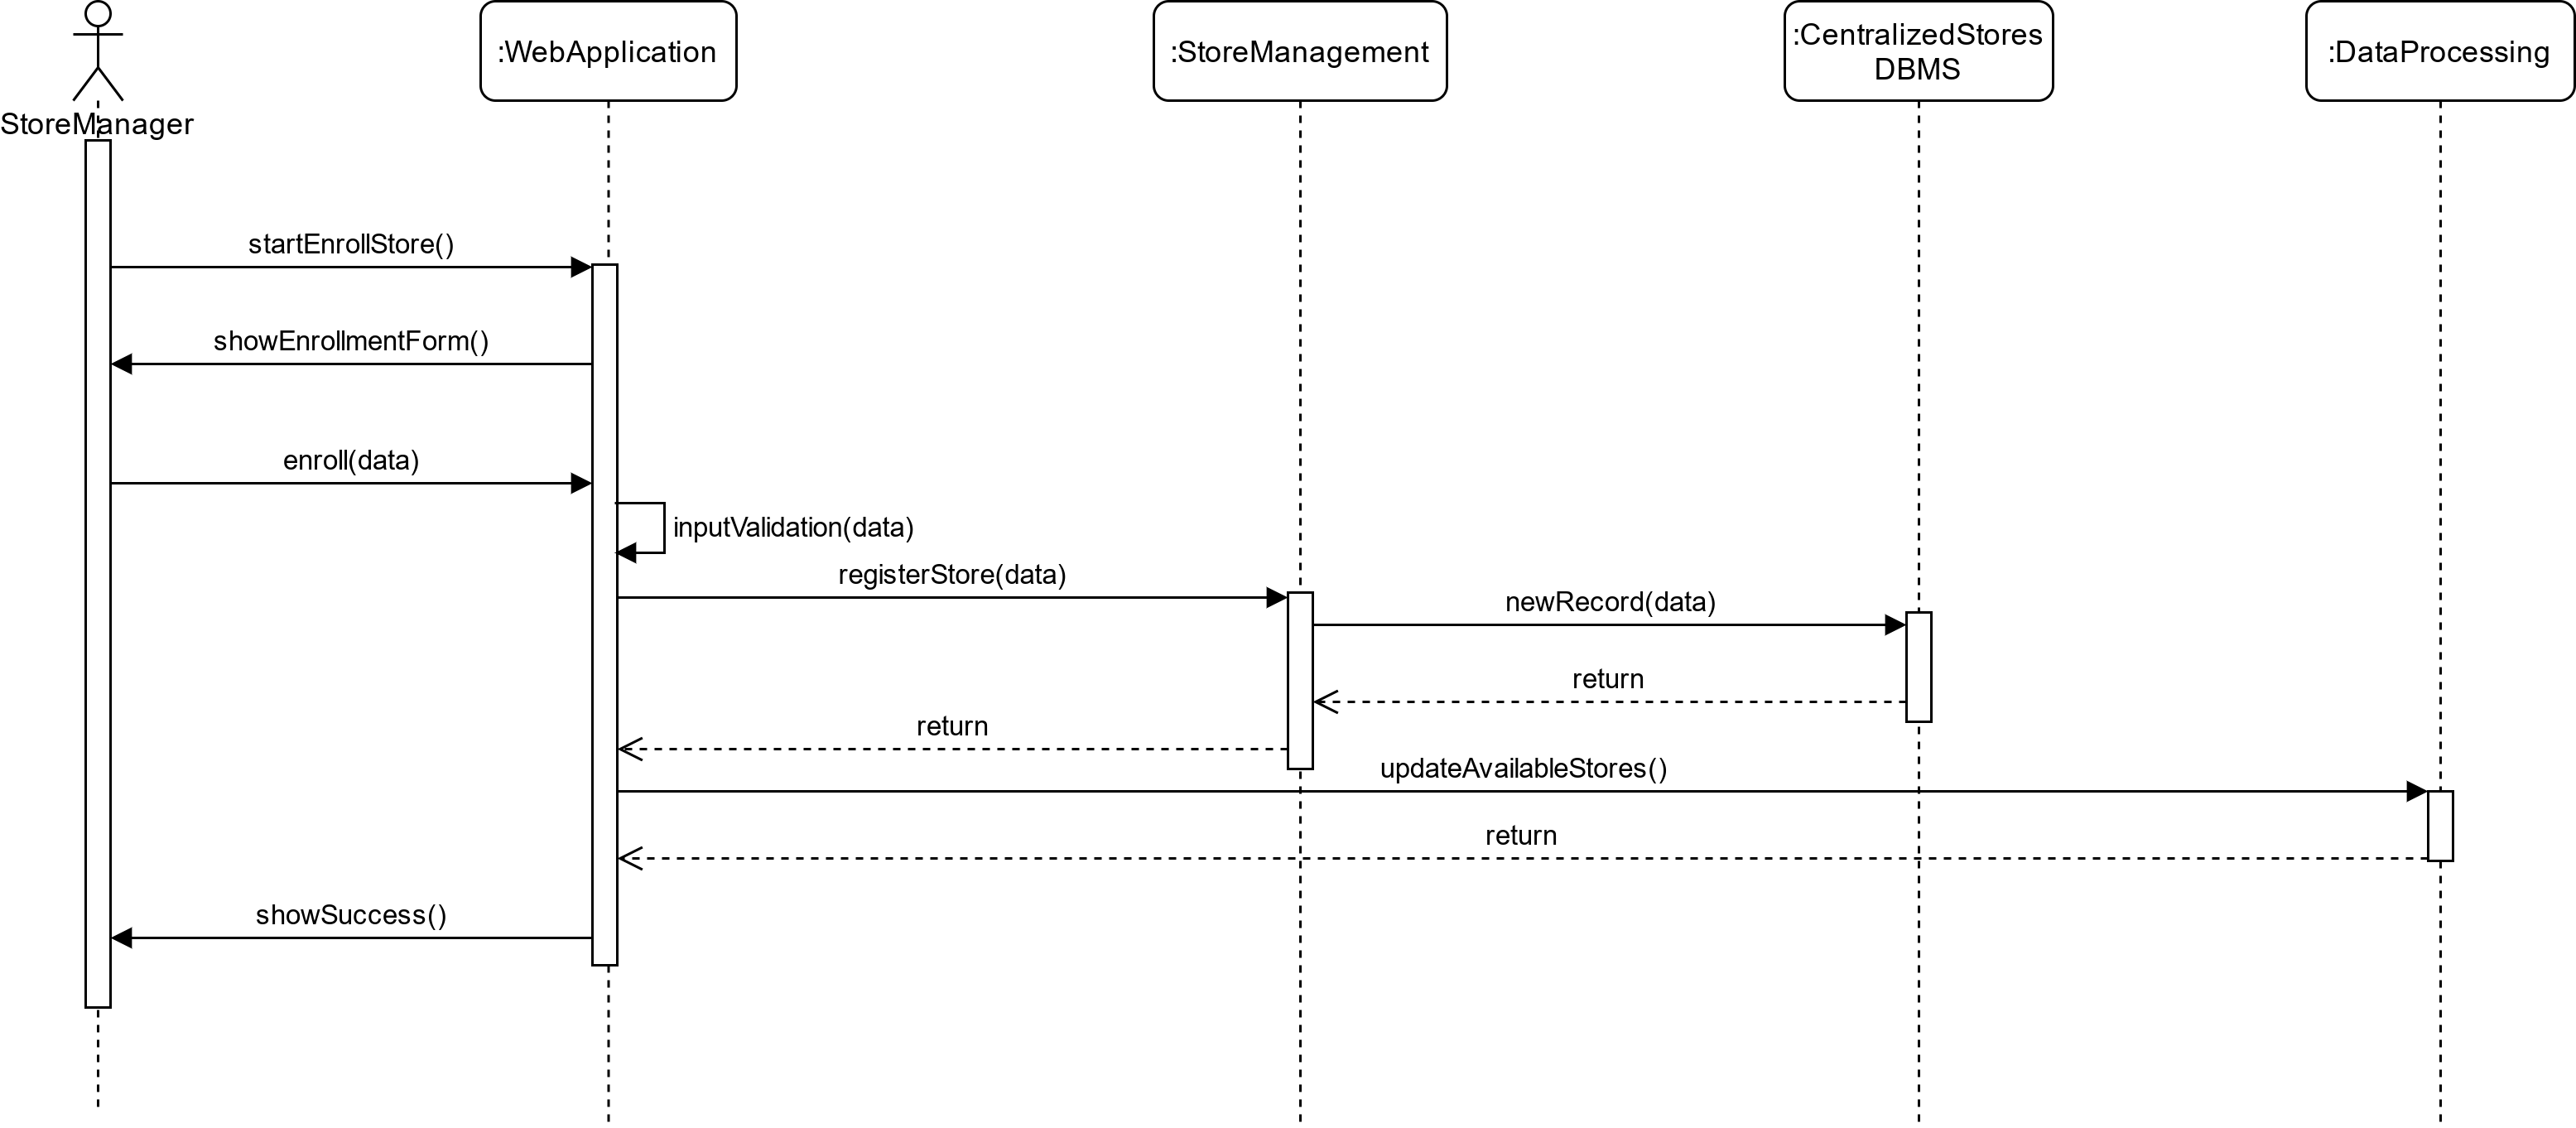
\includegraphics[width=\linewidth]{../Diagrams/Sequence/sequence_store_enroll.png}
	\caption{Sequence Diagram: Store Enrollment procedure}
	\label{fig:sStoreEn}
\end{figure}

\begin{figure}[H]
	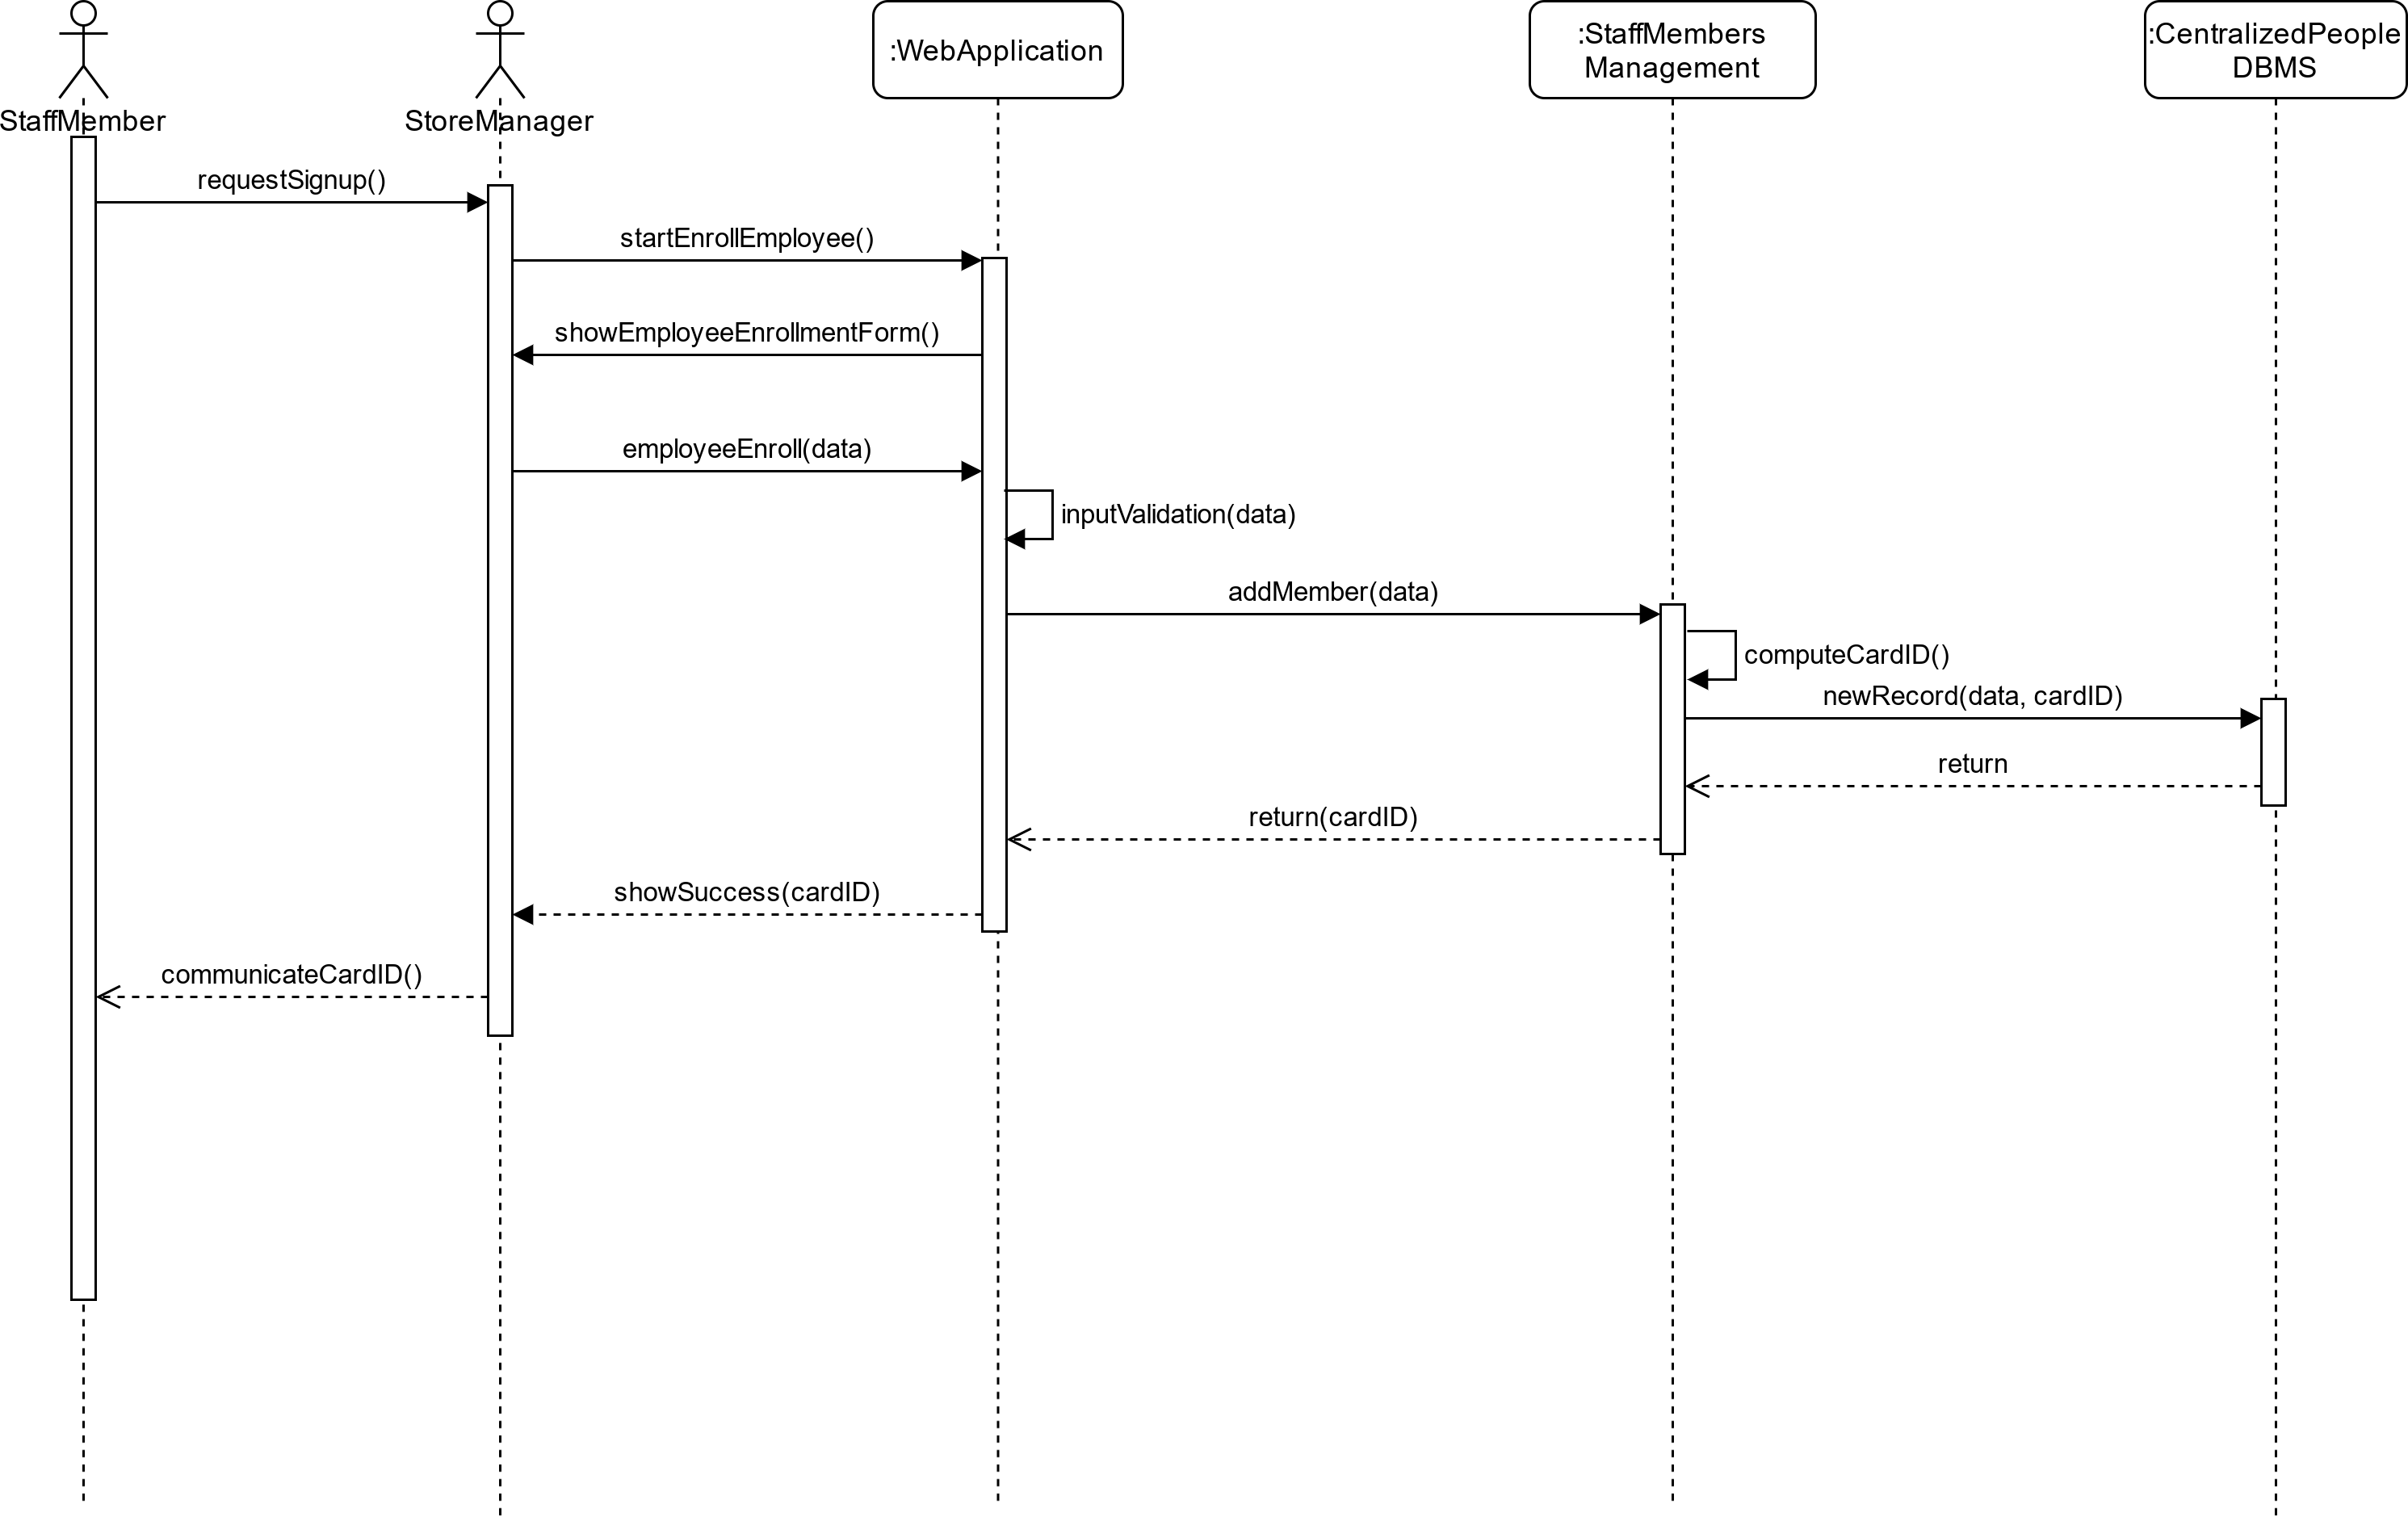
\includegraphics[width=\linewidth]{../Diagrams/Sequence/sequence_staff_enroll.png}
	\caption{Sequence Diagram: Staff Enrollment procedure}
	\label{fig:sStaffEn}
\end{figure}
\begin{figure}[H]
	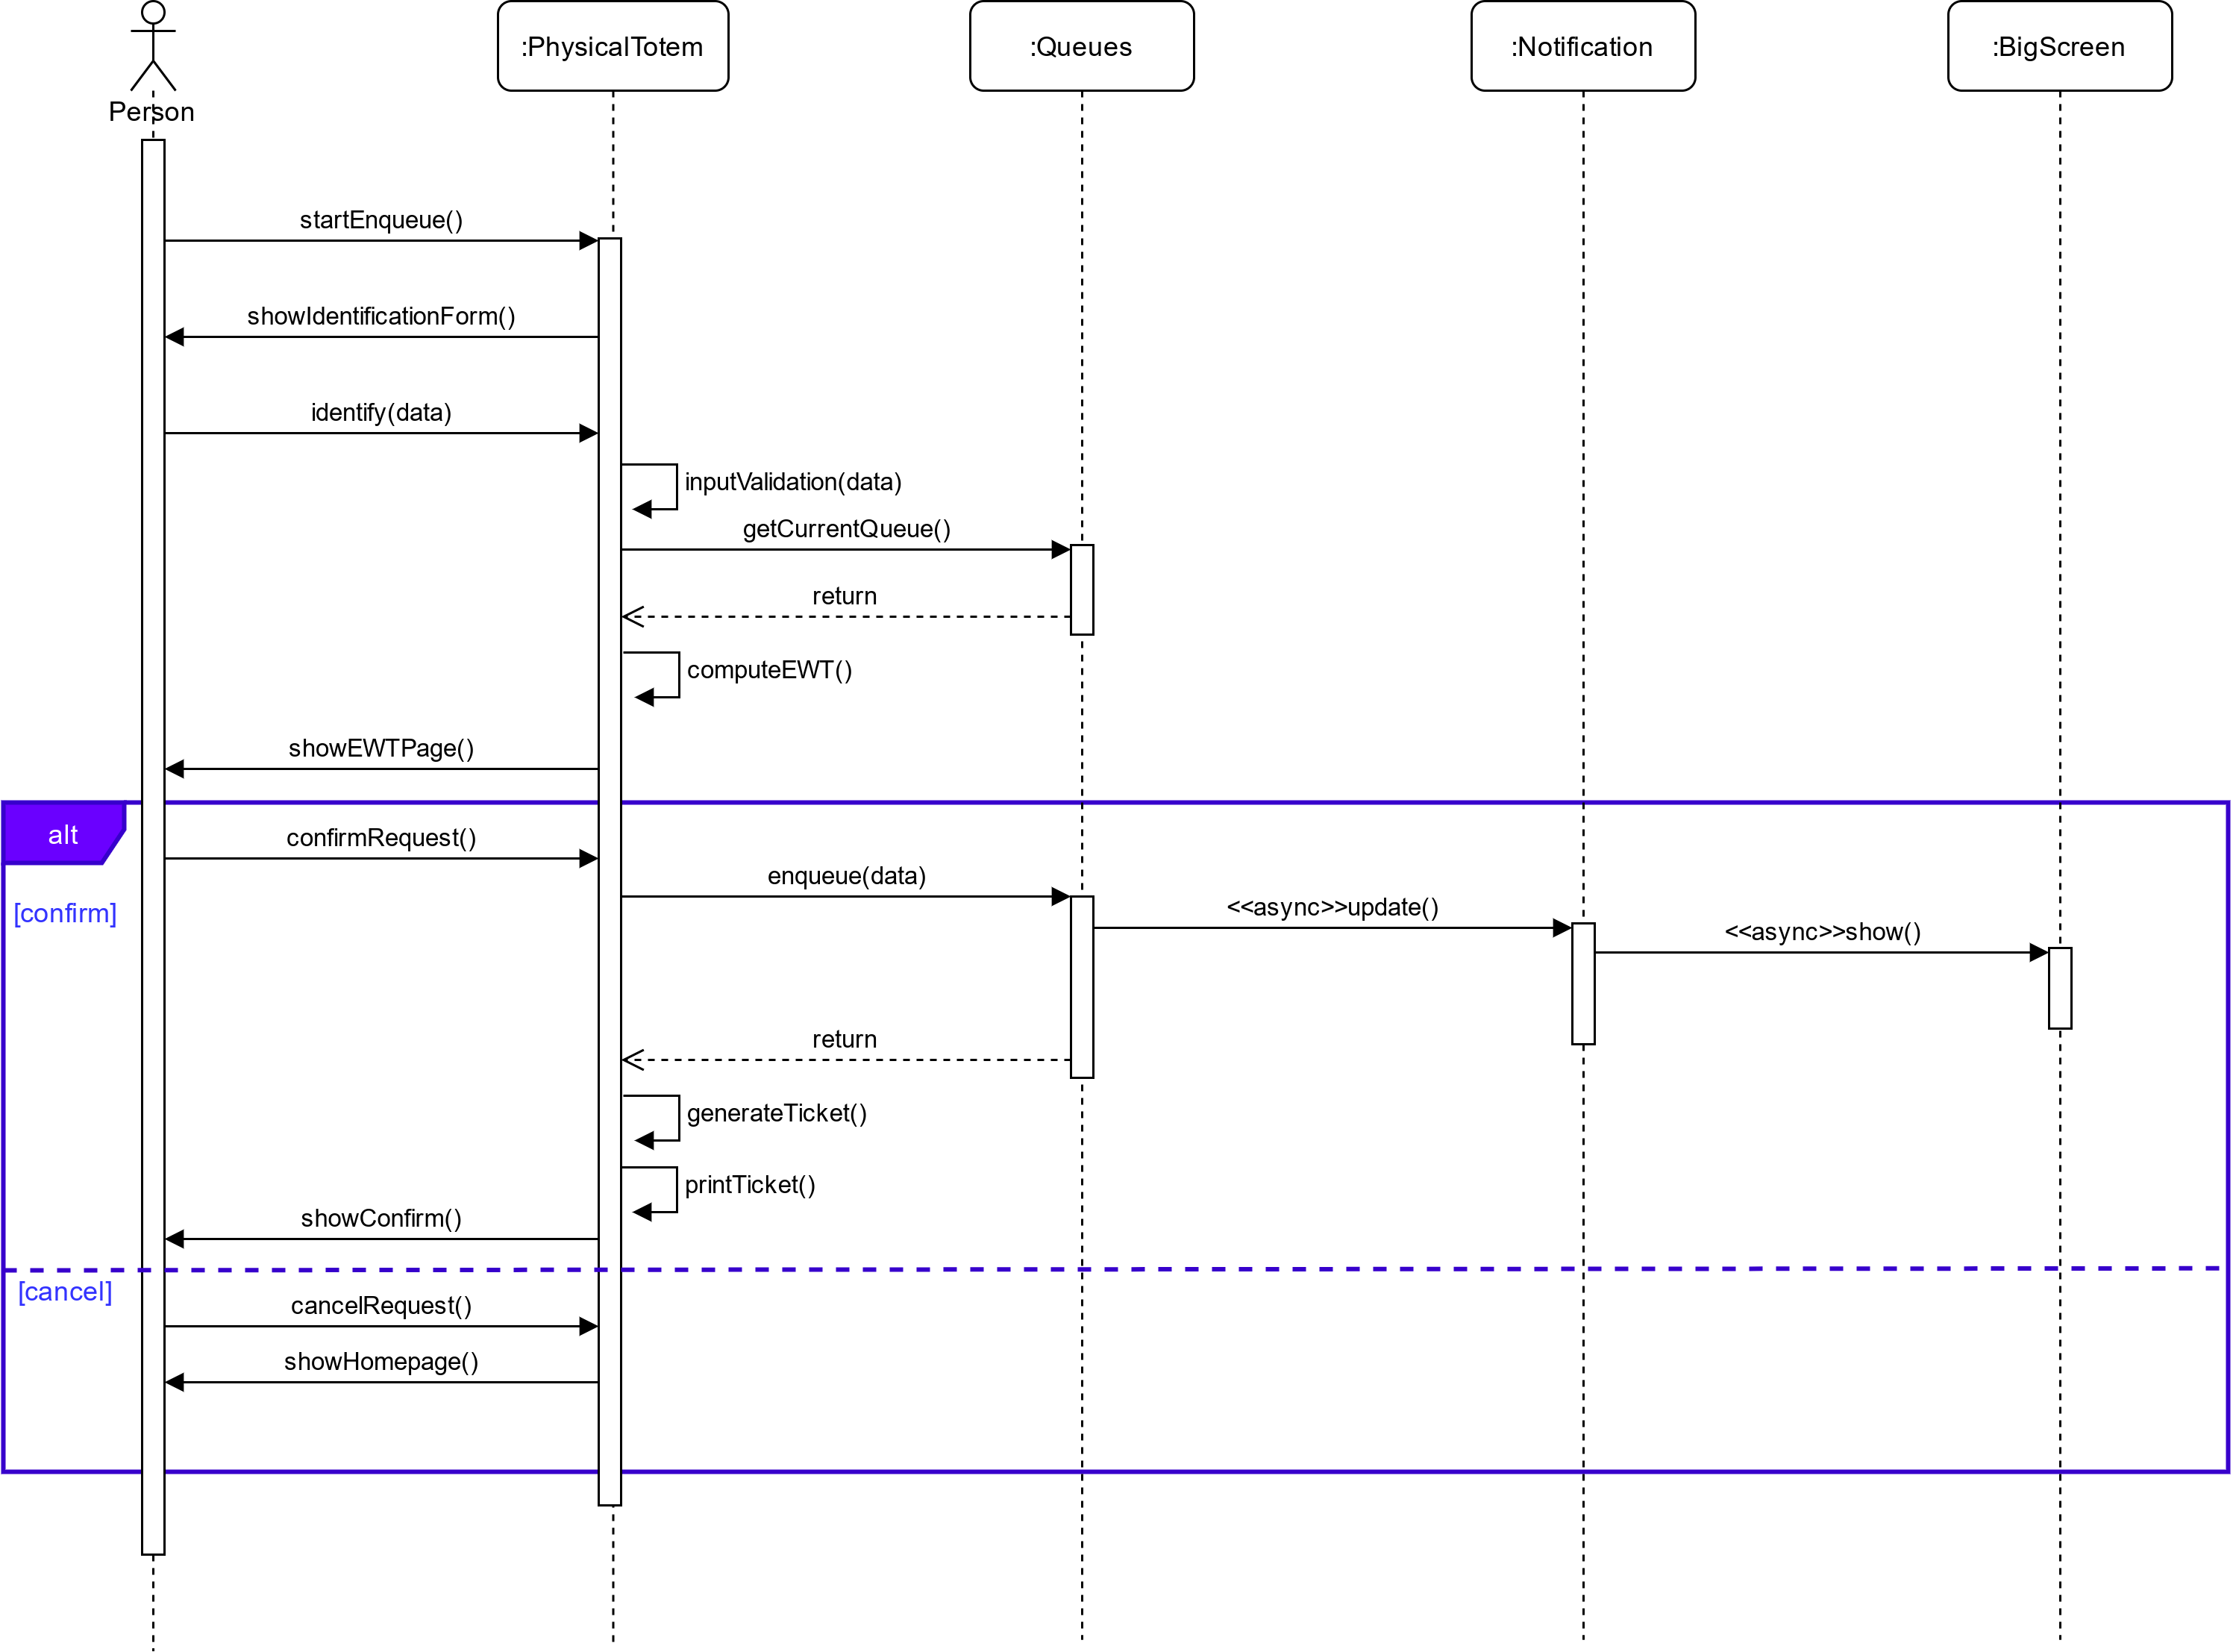
\includegraphics[width=\linewidth]{../Diagrams/Sequence/sequence_totem_enqueue.png}
	\caption{Sequence Diagram: Totem Queueing (physical ticket)}
	\label{fig:sTotemEnq}
\end{figure}

\begin{landscape}

\begin{figure}[H]
	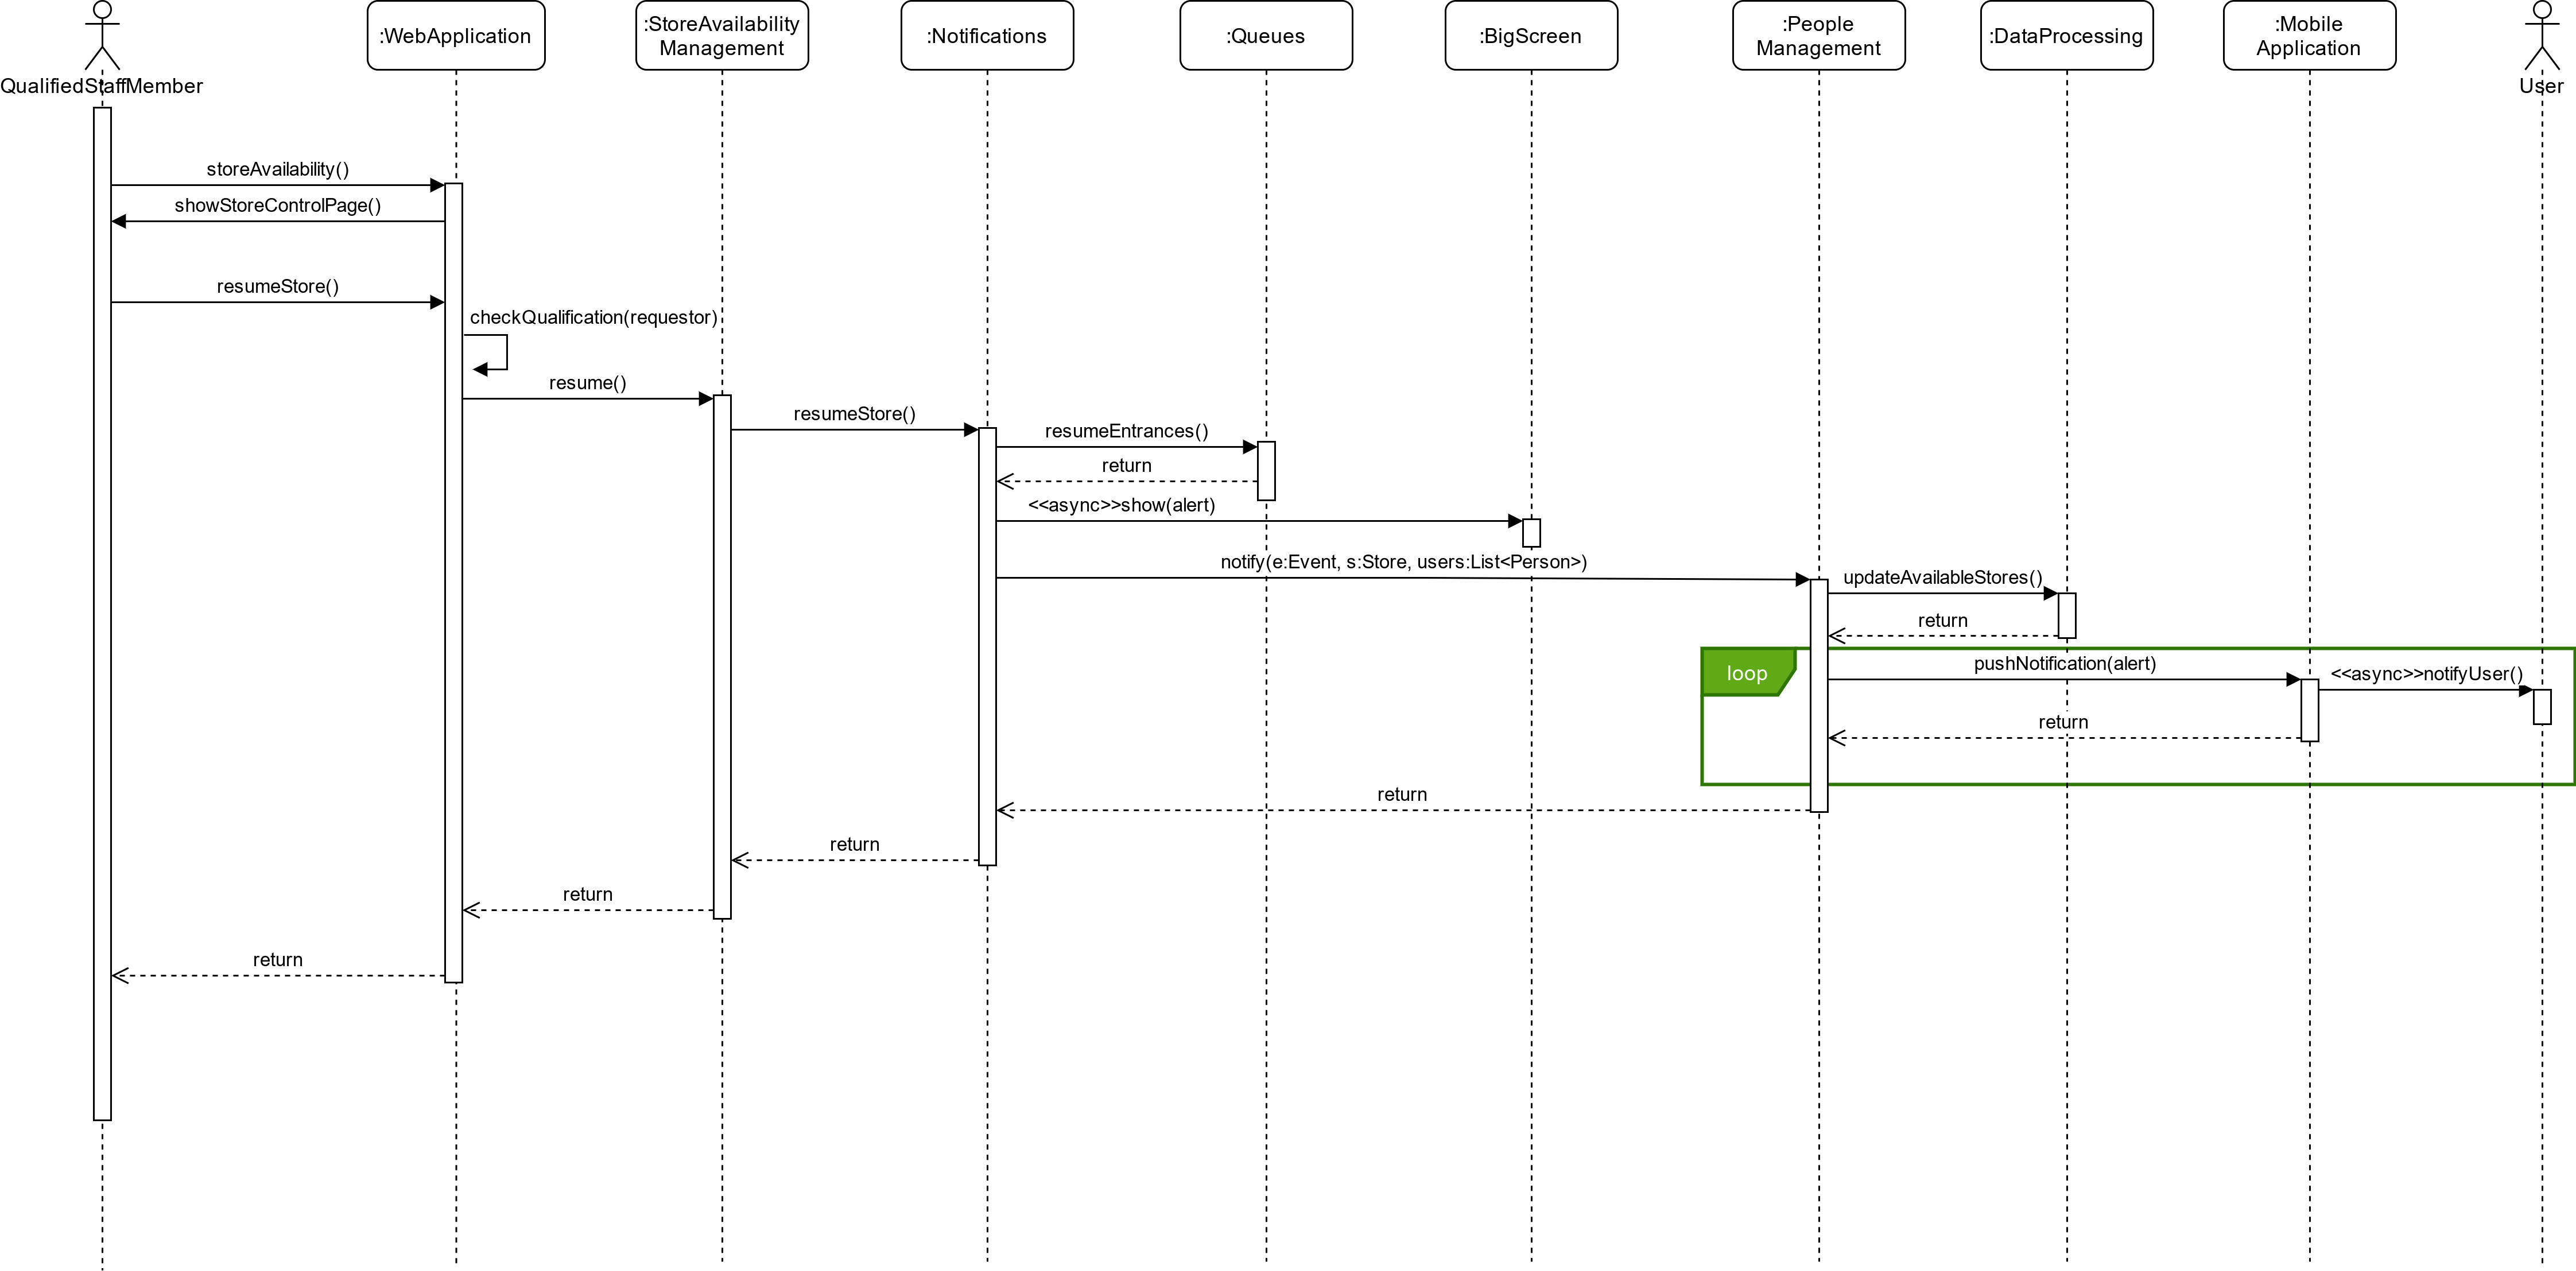
\includegraphics[width=\linewidth]{../Diagrams/Sequence/sequence_store_resume.png}
	\caption{Sequence Diagram: Resuming the Store}
	\label{fig:sStoreRes}
\end{figure}

\begin{figure}[H]
	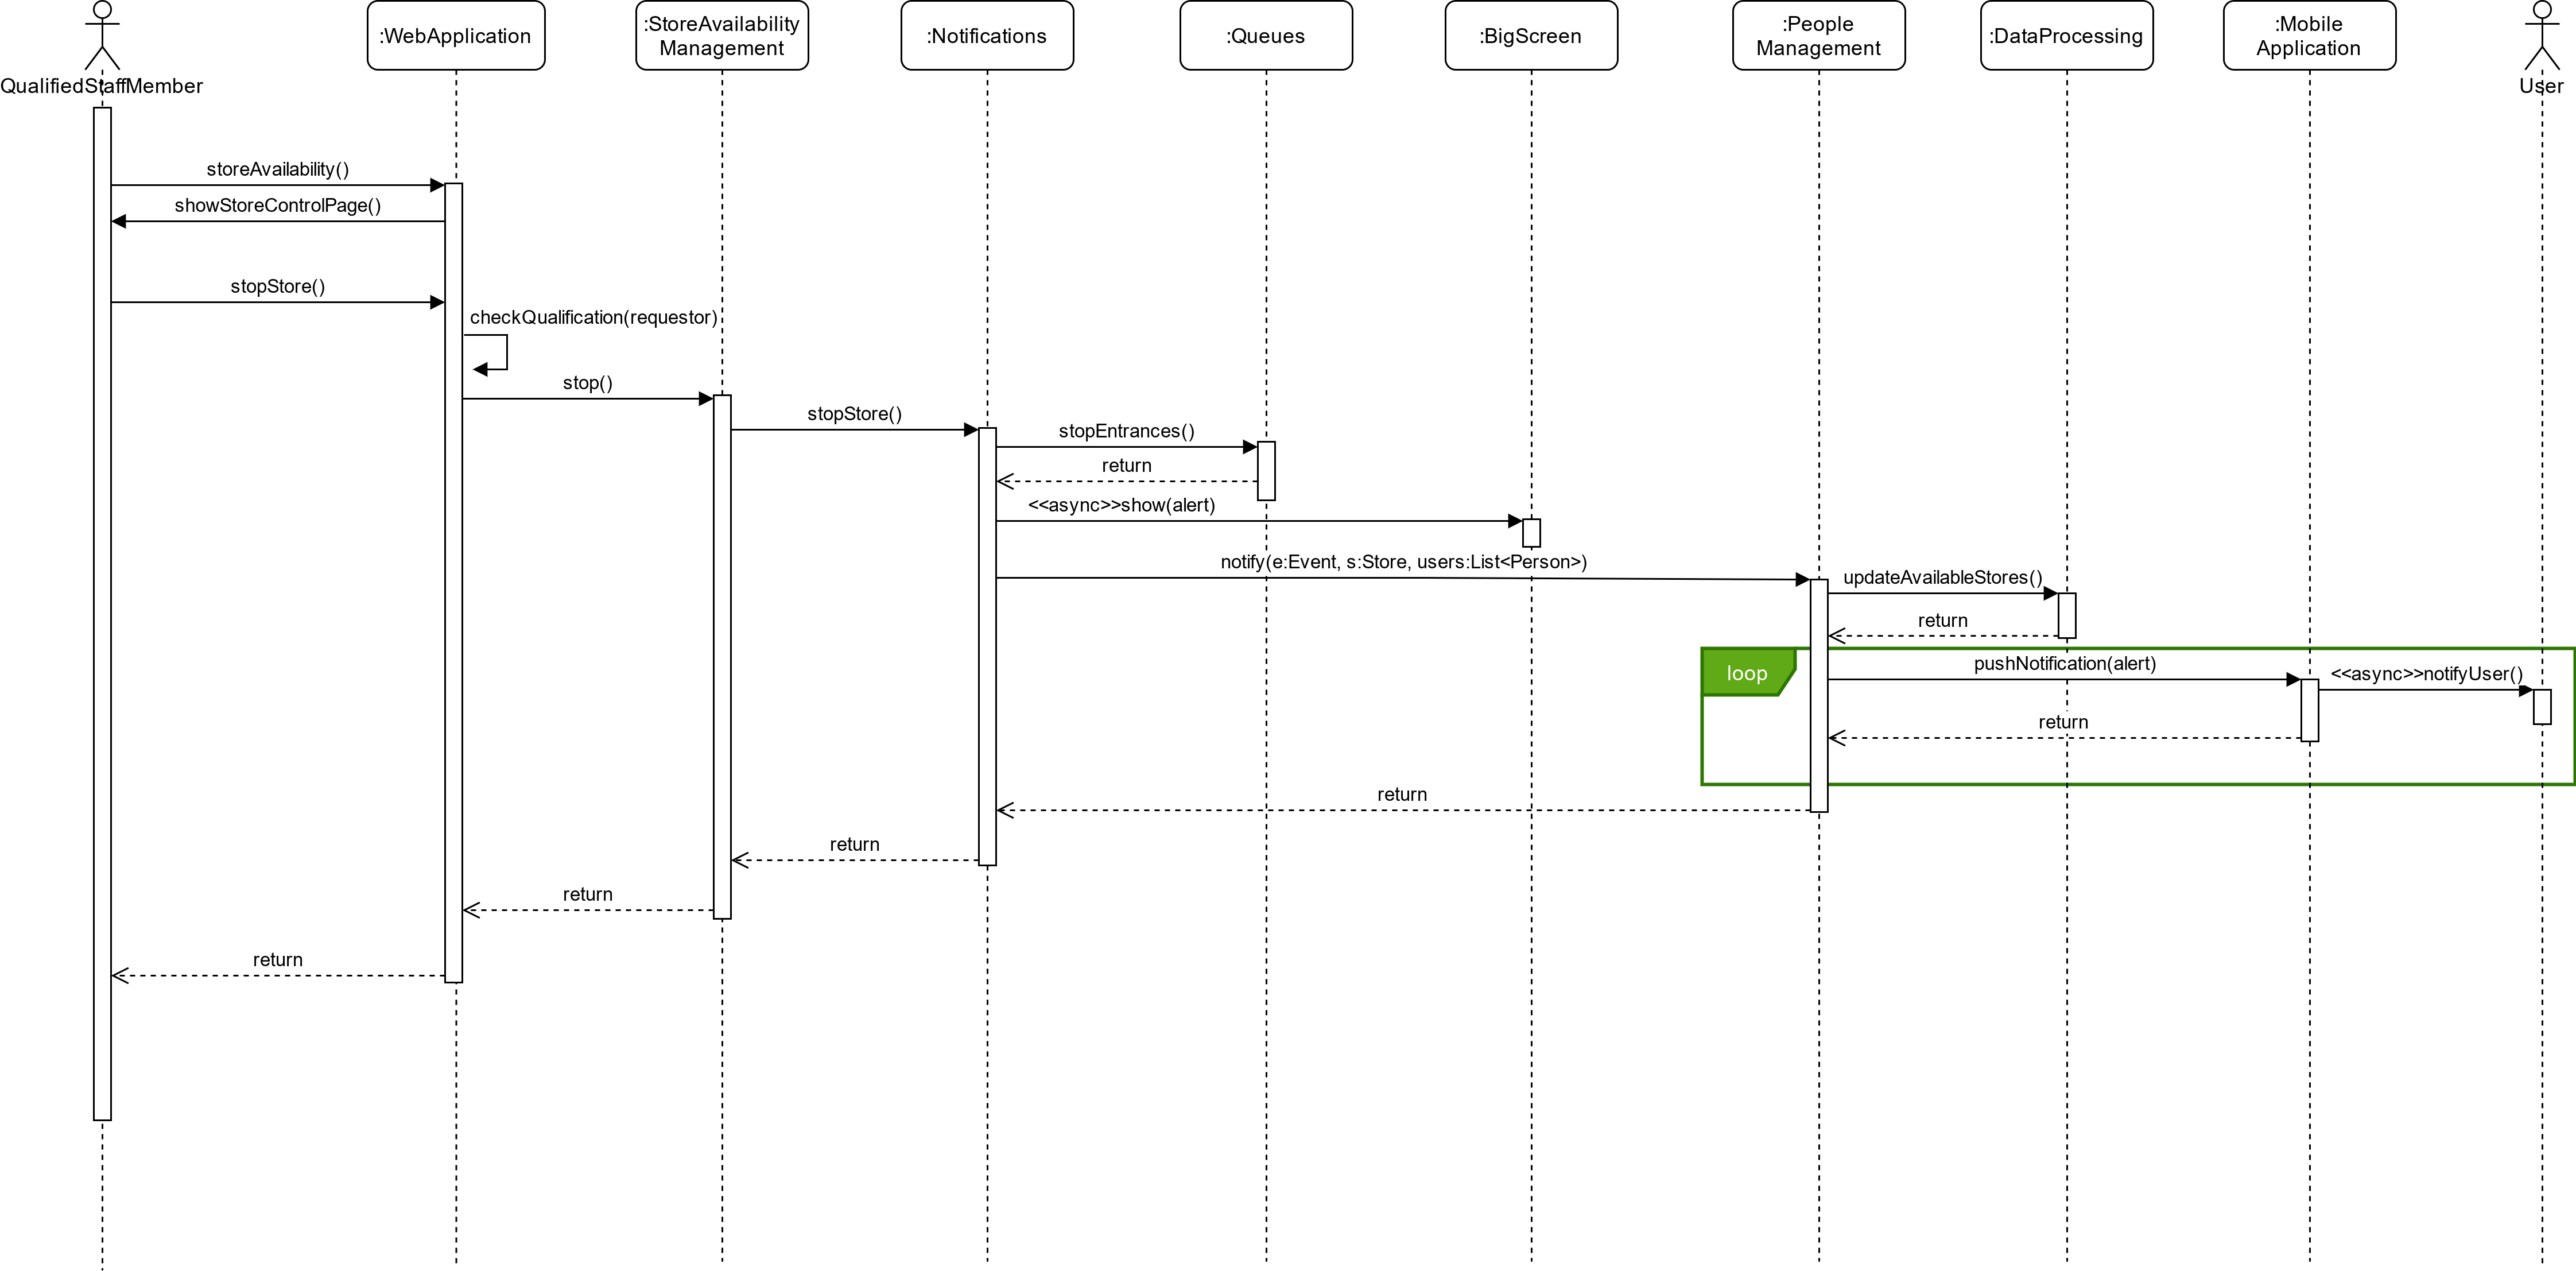
\includegraphics[width=\linewidth]{../Diagrams/Sequence/sequence_store_override.png}
	\caption{Sequence Diagram: Stopping the Store}
	\label{fig:sStoreOver}
\end{figure}

\begin{figure}[H]
	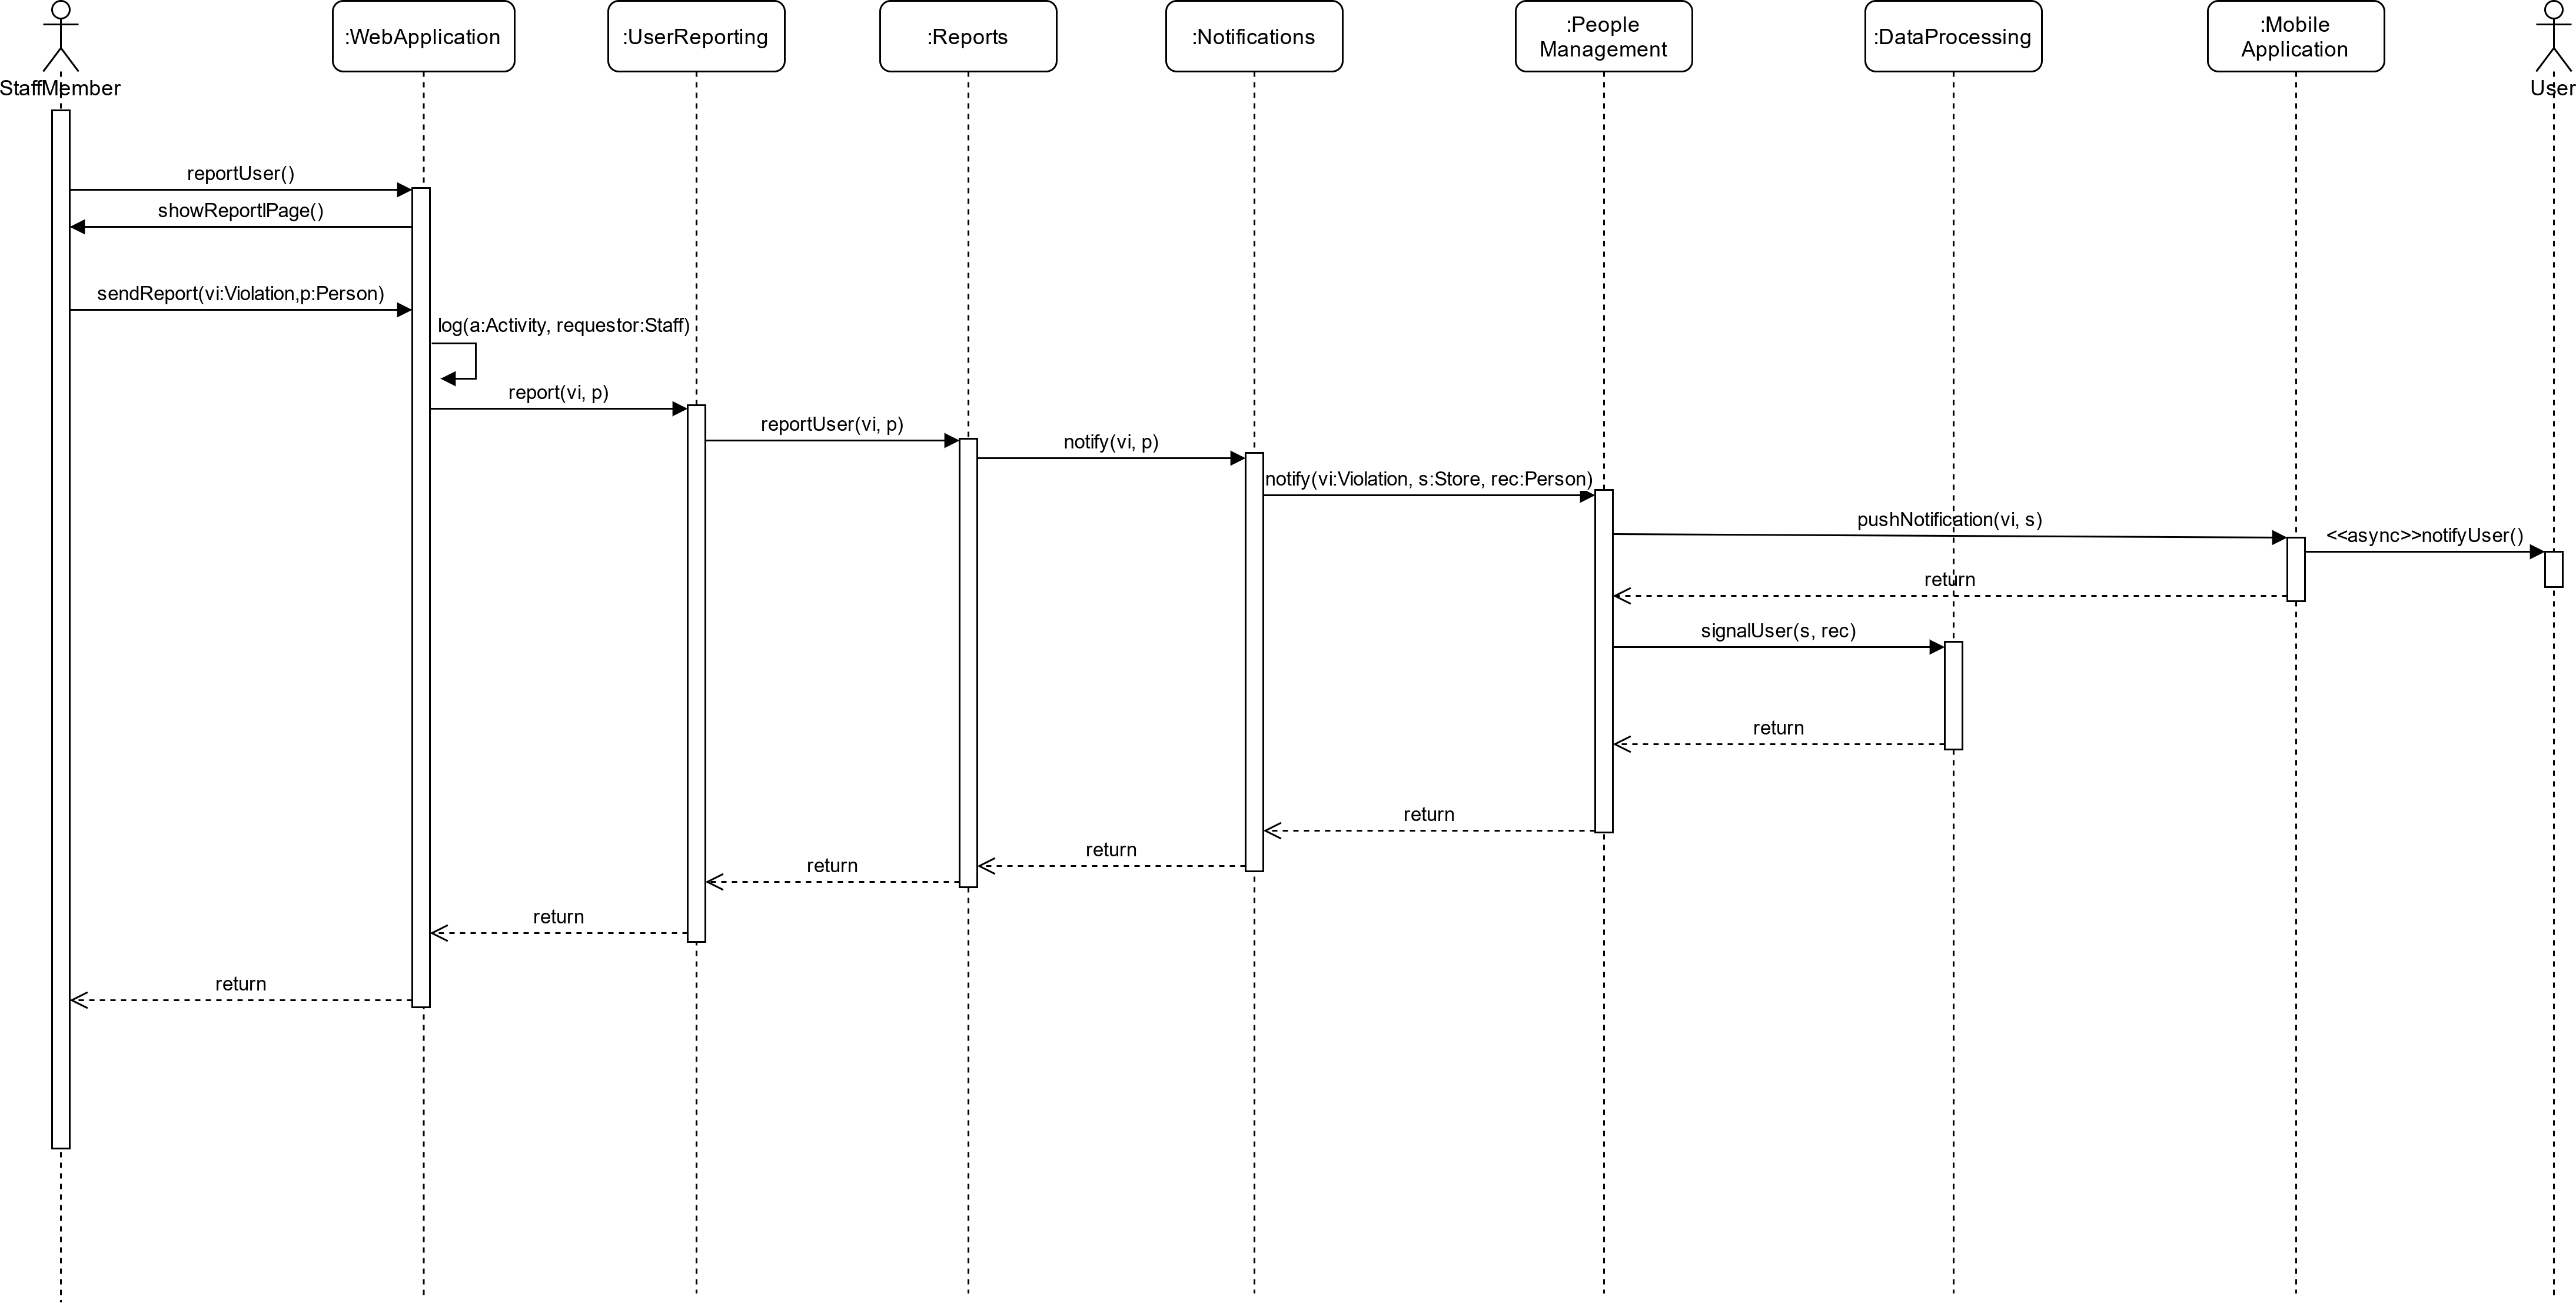
\includegraphics[width=\linewidth]{../Diagrams/Sequence/sequence_user_report.png}
	\caption{Sequence Diagram: Reporting a User}
	\label{fig:sUserRep}
\end{figure}

\begin{figure}[H]
	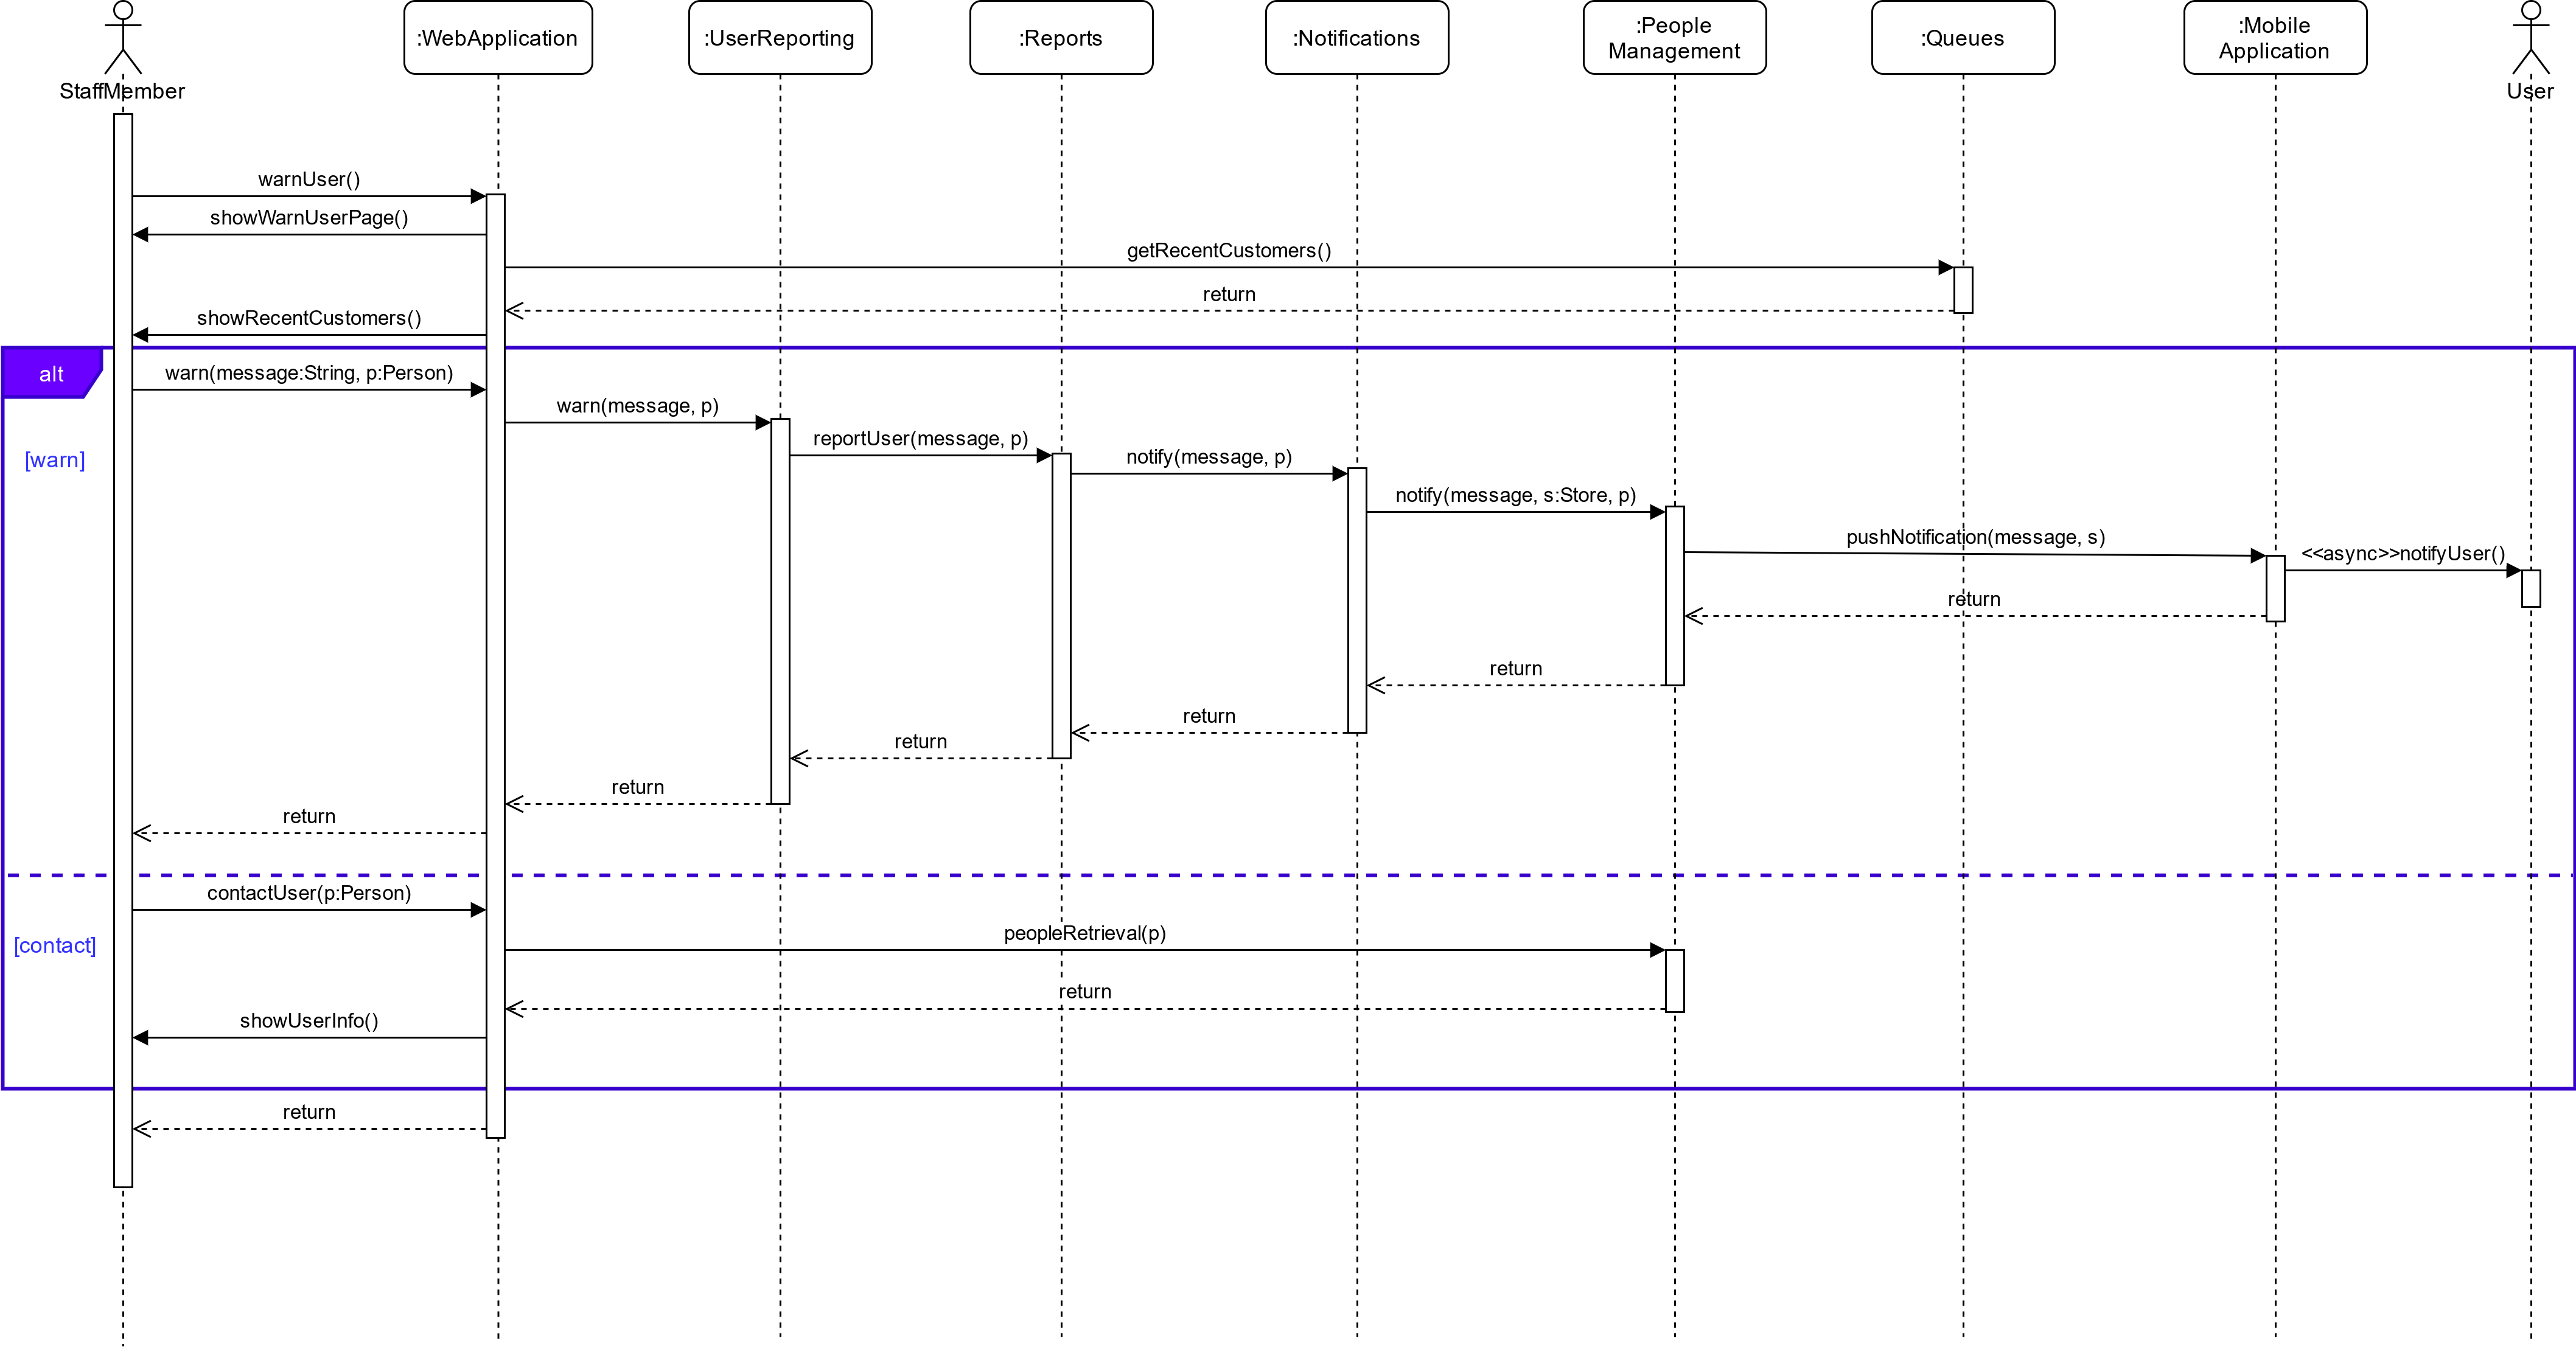
\includegraphics[width=\linewidth]{../Diagrams/Sequence/sequence_user_warn.png}
	\caption{Sequence Diagram: Warning a User}
	\label{fig:sUserWarn}
\end{figure}

\end{landscape}
\subsection{Component interfaces}
\begin{figure}[H]
	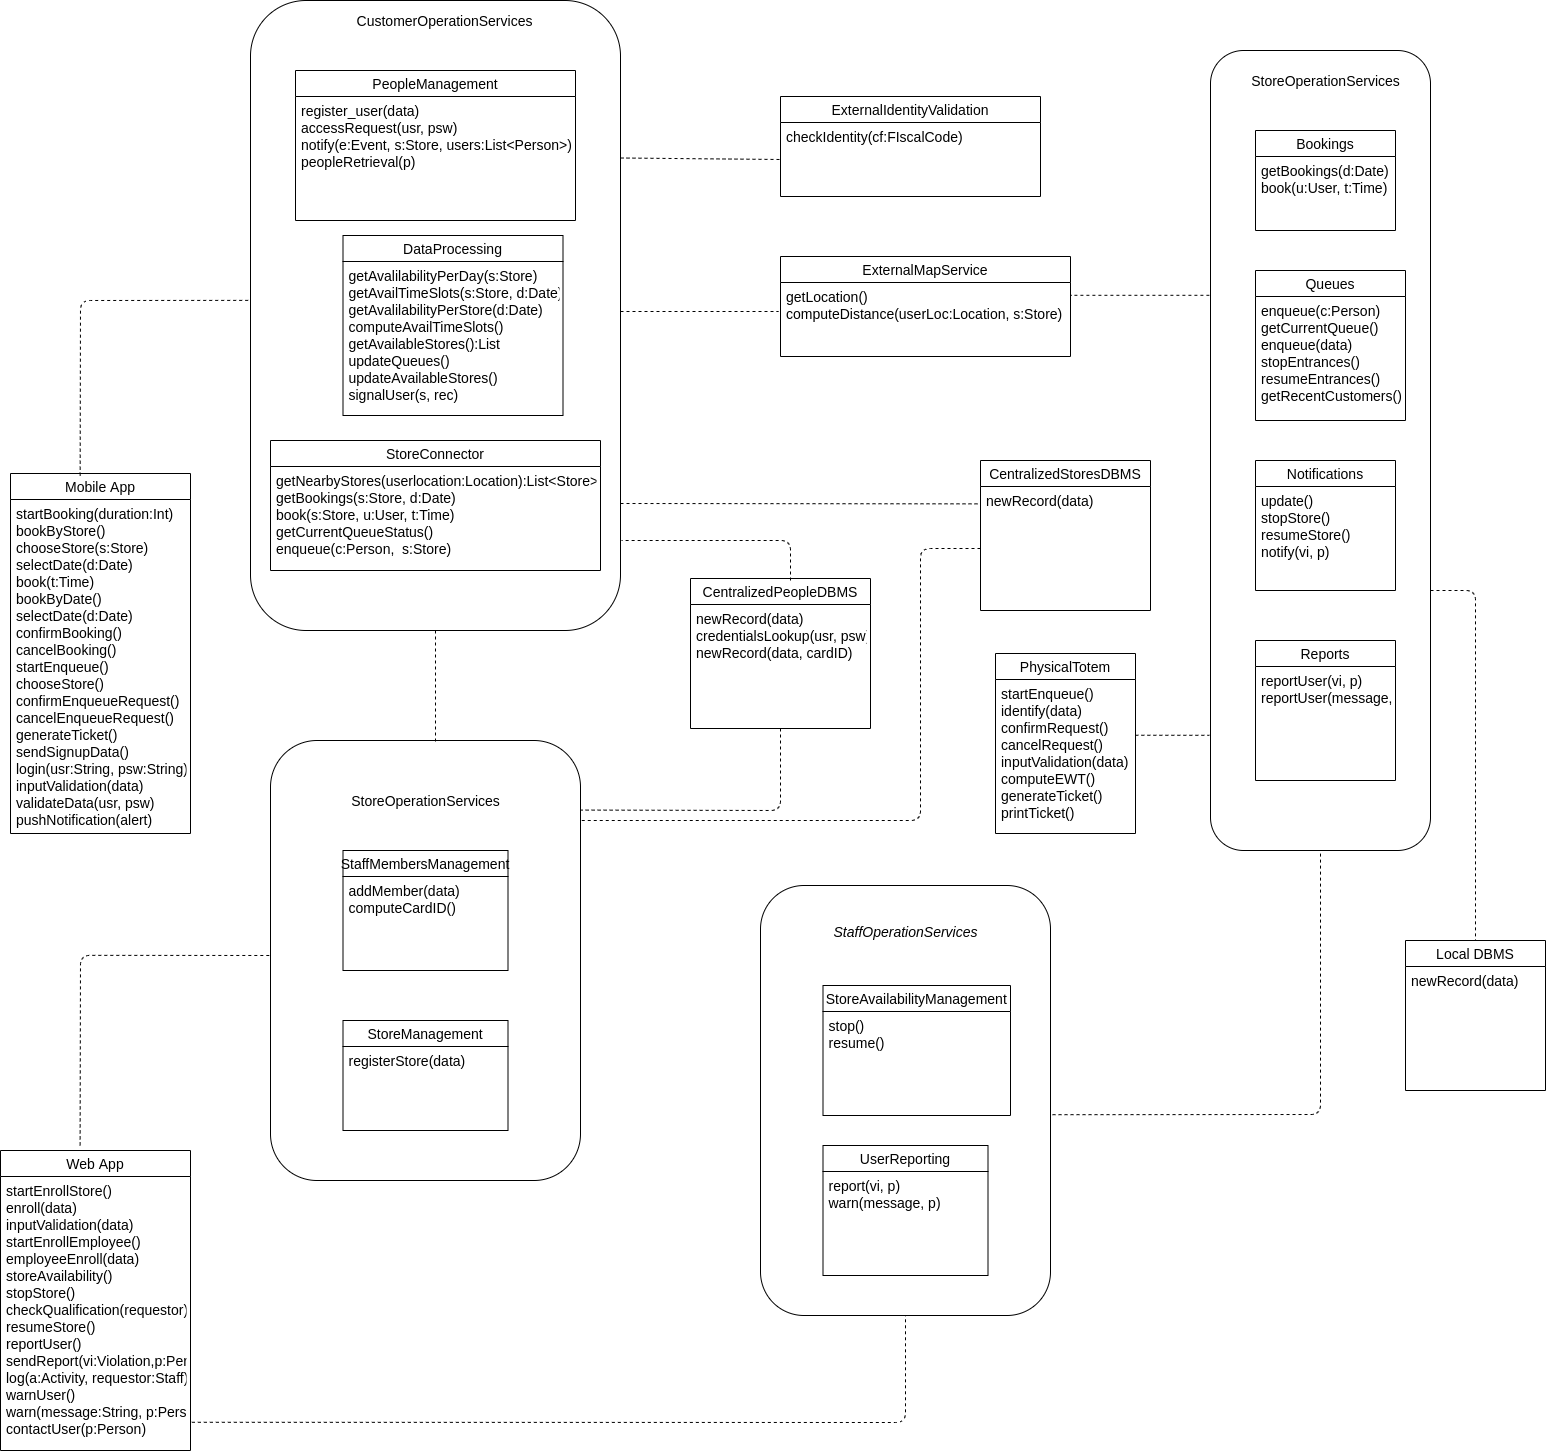
\includegraphics[width=\linewidth]{../Diagrams/Component Interface.png}
	\caption{Component Interface Diagram}
	\label{fig:CompInt}
\end{figure}
\subsection{Selected architectural styles and patterns}
As previously mentioned, a multi-tier client-server architecture has been used to develop CLup in order to promote a major decoupling of the system and to increase the reusability, scalability and
flexibility. CLup servers wait for requests to arrive from clients and then respond to them, server provides clients a standardized transparent interface so that they need not be aware of the specifics of the system that is providing the service.\\
For what concern design patterns, the best suited for this application is MVC: it is a very flexible pattern that massively increase decoupling and simultaneous development through the division of the related program logic into three interconnected elements, Model, View and Controller.
Briefly: \begin{itemize}
	\item Model: The central component of the pattern, Model is the application's dynamic data structure, independent of the user interface, it directly manages the data, logic and rules of the application.
	\item View: This component presents information to the user
	\item Controller: This component is responsible for interpreting the input and manipulating the model based on that input.
	\end{itemize}
A possible way to implement MVC is a combination of Observer, Composite and Strategy patterns:
\begin{itemize}
	\item The model implements the Observer pattern to keep interested objects, typically in the View, updated when state changes occur. In this way it is possible to use different views with the same model or even multiple views at once
	\item GUIs consists of a nested set of a windows, panels and so on. Using Composite, each of those components is a composite or a leaf, when the controller tells the view to update, it only has to tell the top view component and Composite takes care of the rest
	\item The view and controller implement the classic Strategy Pattern, the view is an object that is configured with a strategy. The controller provides the strategy and the view is concerned only with the visual aspects of the application, it delegates to the controller for any decisions about the interface behavior. Using the Strategy pattern also keeps the view decoupled from the model because it is the controller that is responsible for interacting with the model to carry out user requests 
\end{itemize}

\subsection{Other design decisions}
As all the diagrams of the previous sections outline, CLup adopts some particular design decisions worth being discussed. \newline
One of those decision is the way in which the application is distributed. According to the aims of this section, CLup's functionality may be summarized as follows:
\begin{itemize}
    \item Presentation \& User interaction
    \item Flow management \& local business functionality.
\end{itemize}
Let's discuss them in detail.
\paragraph{User interaction}
The \textbf{Presentation \& user interaction} set of functionalities (from now on: PUIF) covers anything from the registration of new components/people (customers, staff members, stores etc.) to the making of a booking, the virtual queueing process and so on. Every single interaction taking place between CLup and its users has to be included here. \newline
We have chosen for these functionalities a \textbf{cost-saving biased trade-off}. We have decided to sacrifice robustness and - eventually - availability of such functionalities in favour of a more affordable and easy-to-implement architecture: one of CLup's main objectives is to become ubiquitous, so to make  increasing the reach of its very primary goal (safer grocery shopping) possible.\newline
In particular, the following aspects have been taken into consideration:
\begin{itemize}
    \item PUIF usually require a stable, huge \textbf{bandwidth} which would have been difficult to get access to in many locations, in case a distributed approach were chosen instead.
    \item PUIF, still being one fundamental functionality, is less vital wrt. FMLBF\footnote{Refer to \ref{def:acronyms}} (see next paragraph for more on this)
    \item A distributed approach for PUIF would require massive infrastructure updates for the majority of stores willing to join the CLup network. This would in turn reduce the number of potential target stores, thus reducing CLup's main goal reach.
    \item In the event of connection loss between central and remote (localized) servers, new bookings and tickets would not be issued for the affected stores. Still, \textbf{already existing ones would not be affected.}
    \begin{itemize}
        \item Similarly, in the event of main servers outage, CLup clients would not be able handle the generation of new booking and tickets, but still, they would be able to serve already generated ones - offline.
    \end{itemize}
\end{itemize}

\paragraph{Local business}
Completely opposite considerations have been made for \textbf{FMLBF}. These functionalities are indeed considered of strong, vital importance and have then been qualified eligible for a distributed architecture requirement. A \textbf{robustness/availability biased trade-off} was in fact chosen, also as a consequence of the following aspects:\newline
\begin{itemize}
    \item FMLBF mainly involve queue management, physical access control to the store, store control, physical ticketing. 
    \item Aforementioned functionalities do not require internet access nor communication with the main servers, provided that the necessary local data structures are put in place.
    \item As a consequence, the communication between main and remote (localized) servers assumes a new less-vital role, in which it allows part of CLup's functionality (booking, virtual queueing...) but \textbf{does not prevent others in the event of failure}.
    \begin{itemize}
        \item Customers would still be able to \textbf{access the store with a valid ticket}, even in case of broadband connection failure
        \item Customers would still be able to \textbf{exit the store scanning} that same ticket
        \item Customers would still be able to get \textbf{physical tickets} outside the store, even during a broadband connection failure event
        \begin{itemize}
            \item This in turns indicates (even though with limitations induced by the number of physical totems present) guarantee of access to the store to a \textbf{non-zero number of people} even during such events.
        \end{itemize}
        \item People flows would still be guaranteed to be handled correctly and consistently \textbf{during and after} the event of broadband connection failure.
        \item Within normal operation conditions, CLup's business logic would require either:
        \begin{itemize}
            \item \textbf{Less costs}, in terms of storage (caches would be needed for a centralized approach), or..
            \item ..\textbf{Less latency} in the processing of customer related events (access, exit etc.).
        \end{itemize}
    \end{itemize}
    \item 

\end{itemize}

\paragraph{Databases}

Given all the considerations above, databases have been split into:
\begin{itemize}
    \item \textbf{Central} databases. Those holding information about general facts, such as the \textbf{Stores} Database, or about entities that are not store-specific: like persons (\textbf{People} Database).
    \item \textbf{Localized} databases. Those holding information about store-specific facts or entities, such as \textbf{Reports, Notifications, Bookings and Tickets} databases.
\end{itemize}

Each store may \textbf{optionally} hold a \textbf{cache} for most relevant central databases entries. 

